\documentclass{abntex2}[
	% -- opções da classe memoir --
	12pt,				% tamanho da fonte
	openright,			% capítulos começam em pág ímpar (insere página vazia caso preciso)
	twoside,			% para impressão em recto e verso. Oposto a oneside
	a4paper,			% tamanho do papel. 
	% -- opções da classe abntex2 --
	chapter=TITLE,		% títulos de capítulos convertidos em letras maiúsculas
	section=TITLE,		% títulos de seções convertidos em letras maiúsculas
	subsection=TITLE,	% títulos de subseções convertidos em letras maiúsculas
	subsubsection=TITLE,% títulos de subsubseções convertidos em letras maiúsculas
	% -- opções do pacote babel --
	english,			% idioma adicional para hifenização
	brazil				% o último idioma é o principal do documento
]

% ---
% Pacotes básicos 
% ---
\usepackage{lmodern}			% Usa a fonte Latin Modern	
\usepackage[T1]{fontenc}		% Selecao de codigos de fonte.
\usepackage[utf8]{inputenc}		% Codificacao do documento (conversão automática dos acentos)
\usepackage{lastpage}			% Usado pela Ficha catalográfica
\usepackage{indentfirst}		% Indenta o primeiro parágrafo de cada seção.
\usepackage{color}				% Controle das cores
\usepackage{graphicx}			% Inclusão de gráficos
\usepackage{microtype} 			% para melhorias de justificação
\usepackage{mathtools}
\usepackage{pgfplots}
\usepackage{tikz}
\usetikzlibrary{calc}
\usetikzlibrary{arrows}
\usepackage{amsmath}
% \usepackage{natbib}
\usepackage{subcaption}
\usepackage{longtable}
\usepackage{booktabs} % For prettier tables
\usepackage{siunitx} % Required for alignment
\usepackage{bm} % Matemática em bold
\usepackage{siunitx} % Required for alignment
\usepackage{booktabs} % For prettier tables
\usepackage{adjustbox}
\usepackage{todonotes}
\usepackage{float}

% \documentclass{article}

% \usepackage{biblatex}
% \addbibresource{references.bib}

\sisetup{
  round-mode          = places, % Rounds numbers
  round-precision     = 2, % to 2 places
}

% ---
% Pacotes de citações
% ---
\usepackage[brazilian,hyperpageref]{backref}	 % Paginas com as citações na bibl
\usepackage[alf]{abntex2cite}	% Citações padrão ABNT

% ---
% Configurações de aparência do PDF final

% alterando o aspecto da cor azul
\definecolor{blue}{RGB}{41,5,195}

% informações do PDF
\makeatletter
\hypersetup{
     	%pagebackref=true,
		pdftitle={\@title}, 
		pdfauthor={\@author},
    	pdfsubject={\imprimirpreambulo},
	    pdfcreator={LaTeX with abnTeX2},
		pdfkeywords={abnt}{latex}{abntex}{abntex2}{trabalho acadêmico}, 
% 		colorlinks=true,       		% false: boxed links; true: colored links
    	linkcolor=blue,          	% color of internal links
    	citecolor=blue,        		% color of links to bibliography
    	filecolor=magenta,      		% color of file links
		urlcolor=blue,
		bookmarksdepth=4
}
\makeatother
% --- 

% ---
% Configurações do pacote backref
% Usado sem a opção hyperpageref de backref
\renewcommand{\backrefpagesname}{Citado na(s) página(s):~}
% Texto padrão antes do número das páginas
\renewcommand{\backref}{}
% Define os textos da citação
\renewcommand*{\backrefalt}[4]{
	\ifcase #1 %
		Nenhuma citação no texto.%
	\or
		Citado na página #2.%
	\else
		Citado #1 vezes nas páginas #2.%
	\fi}%
% --- 
% Espaçamentos entre linhas e parágrafos 
% --- 

% O tamanho do parágrafo é dado por:
\setlength{\parindent}{1.3cm}

% Controle do espaçamento entre um parágrafo e outro:
\setlength{\parskip}{0.2cm}  % tente também \onelineskip

% ---
% compila o indice
% ---
\makeindex
% ---

% ---
% Informações de dados para CAPA e FOLHA DE ROSTO
% ---
\titulo{REDES NEURAIS ARTIFICIAIS PARA PREDIÇÃO DAS PROPRIEDADES DE TRANSPORTE DE VALE EM NANOFITAS DE GRAFENO}
\autor{Pablo Rhuam Cavalcante Silva}
\local{Brasil}
\data{\today}
\orientador{Dario Andres Bahamon Ardila}
\coorientador{Leandro A. Silva}

\instituicao{%
  Universidade Presbiteriana Mackenzie
  \par
%   Faculdade de Arquitetura da Informação
%   \par
  Programa de Pós-Graduação em Engenharia Elétrica e Computação}
\tipotrabalho{Dissertação (Mestrado)}
% O preambulo deve conter o tipo do trabalho, o objetivo, 
% o nome da instituição e a área de concentração 
\preambulo{Dissertação apresentada à Universidade Presbiteriana Mackenzie como requisito parcial para a obtenção do título de Mestre em Engenharia Elétrica e Computação.}
% ---

\begin{document}

% Seleciona o idioma do documento (conforme pacotes do babel)
%\selectlanguage{english}
\selectlanguage{brazil}

% Retira espaço extra obsoleto entre as frases.
\frenchspacing 

\imprimircapa

\imprimirfolhaderosto*

\begin{fichacatalografica}
	\sffamily
	\vspace*{\fill}					% Posição vertical
	\begin{center}					% Minipage Centralizado
	\fbox{\begin{minipage}[c][8cm]{13.5cm}		% Largura
	\small
	\imprimirautor
	%Sobrenome, Nome do autor
	
	\hspace{0.5cm} \imprimirtitulo  / \imprimirautor. --
	\imprimirlocal, \imprimirdata-
	
% 	\hspace{0.5cm} \pageref{LastPage} p. : il. (algumas color.) ; 30 cm.\\
	
	\hspace{0.5cm} \imprimirorientadorRotulo~\imprimirorientador\\ 
    \hspace{0.5cm} \imprimircoorientadorRotulo~\imprimircoorientador\\
	\hspace{0.5cm}
	\parbox[t]{\textwidth}{\imprimirtipotrabalho~--~\imprimirinstituicao,
	\imprimirdata.}\\
	
	\hspace{0.5cm}
		1. grafeno
		2. rede neural artificial
		2. mlp
		I. Orientador
		II. Universidade Presbiteriana Mackenzie
		III. Programa de Pós-Graduação em Engenharia Elétrica e Computação
		IV. REDES NEURAIS ARTIFICIAIS PARA PREDIÇÃO DAS PROPRIEDADES DE TRANSPORTE DE VALE EM NANOFITAS DE GRAFENO 			
	\end{minipage}}
	\end{center}
\end{fichacatalografica}
% ---
% Inserir folha de aprovação
% ---
\begin{folhadeaprovacao}

  \begin{center}
    {\ABNTEXchapterfont\large\imprimirautor}

    \vspace*{\fill}\vspace*{\fill}
    \begin{center}
      \ABNTEXchapterfont\bfseries\Large\imprimirtitulo
    \end{center}
    \vspace*{\fill}
    
    \hspace{.45\textwidth}
    \begin{minipage}{.5\textwidth}
        \imprimirpreambulo
    \end{minipage}%
    \vspace*{\fill}
   \end{center}
        
   Trabalho aprovado. \imprimirlocal, 24 de junho de 2019:

   \assinatura{\textbf{\imprimirorientador} \\ Orientador 1} 
   \assinatura{\textbf{\imprimircoorientador} \\ Coorientador} 
   \assinatura{\textbf{Professor} \\ Convidado 1}
   \assinatura{\textbf{Professor} \\ Convidado 2}
   %\assinatura{\textbf{Professor} \\ Convidado 3}
   %\assinatura{\textbf{Professor} \\ Convidado 4}
      
   \begin{center}
    \vspace*{0.5cm}
    {\large\imprimirlocal}
    \par
    {\large\imprimirdata}
    \vspace*{1cm}
  \end{center}
  
\end{folhadeaprovacao}

% \begin{dedicatoria}
%   \vspace*{\fill}
%   \centering
%   \noindent
%   \textit{ Este trabalho é dedicado ...} \vspace*{\fill}
% \end{dedicatoria}

% \begin{agradecimentos}
% txtxtxtxtxt

% \end{agradecimentos}

% \begin{epigrafe}
%     \vspace*{\fill}
% 	\begin{flushright}
% % 		\textit{``Não vos amoldeis às estruturas deste mundo, \\
% % 		mas transformai-vos pela renovação da mente, \\
% % 		a fim de distinguir qual é a vontade de Deus: \\
% % 		o que é bom, o que Lhe é agradável, o que é perfeito.\\
% % 		(Bíblia Sagrada, Romanos 12, 2)}
% 		\textit{``txt, \\
% 		txt txt. \\
% 		(Bíblia Sagrada, Romanos 12, 2)}
% 	\end{flushright}
% \end{epigrafe}

% \bibliography{references_abstract.bib}

% resumo em português
\setlength{\absparsep}{18pt} % ajusta o espaçamento dos parágrafos do resumo
% \begin{resumo}
% % Vários estudos independentes mostraram que as propriedades eletrônicas do grafeno, como a condutância e transmissão por vale, variam de acordo com as características físicas da fita de grafeno. Ou seja, fitas mais/menos largas, mais/menos compridas e com mais ou menos deformações gaussianas resultam em diferentes valores de condutância e transmissão por vale. O presente trabalho apresenta a modelagem de rede neural artificial capaz de simular e predizer a correlação destas e outras configurações e seus efeitos nas propriedades eletrônicas. Conclui-se que é conveniente e fácil de usar redes neurais artificiais em experimentos numéricos para revisar os efeitos das diferentes configurações físicas de nanofitas de grafeno em relação a sua condutância elétrica e transmissão por vale.

%  \textbf{Palavras-chave}: grafeno. mlp. redes neurais artificiais. transporte eletrônico
% %  Segundo a \citeonline[3.1-3.2]{NBR6028:2003}, o resumo deve ressaltar o
% %  objetivo, o método, os resultados e as conclusões do documento. A ordem e a extensão
% %  destes itens dependem do tipo de resumo (informativo ou indicativo) e do
% %  tratamento que cada item recebe no documento original. O resumo deve ser
% %  precedido da referência do documento, com exceção do resumo inserido no
% %  próprio documento. (\ldots) As palavras-chave devem figurar logo abaixo do
% %  resumo, antecedidas da expressão Palavras-chave:, separadas entre si por
% %  ponto e finalizadas também por ponto.

% %  \textbf{Palavras-chave}: latex. abntex. editoração de texto.
% \end{resumo}

% resumo em inglês
\begin{resumo}[Abstract]
The control of the valley degree of freedom of electrons (valleytronics)  has recently emerged as a promising technology for the next generation of electronic devices; this quantum  number naturally appears in periodic solids with  degenerated local minima and maxima at inequivalent  points of the Brillouin zone. Similar to spintronics, the applicability of valleytronics relies on the electric generation, control and detection of valley currents \citeauthor{Valley2D}; %in this context, 2D materials with hexagonal lattices such as graphene and transition metal dichalcogenides offer two valleys (K and K’) well separated in momentum space that can be accessed by optical \cite{PhysRevB.77.235406,Cao:2012fk}, magnetic \cite{PhysRevLett.113.266804, PhysRevLett.114.037401} and mechanical means \cite{nl400872q,7b01663}. For example, it has been observed that under broken spatial inversion symmetry these systems generate valley-dependent optical selection rules \cite{Lee:2016kx} and dissipation less topological valley current \cite{Gorbachev448}. However, despite the success achieved, this approach is limited to high quality samples with perfect alignment of the layers. On the other hand, electrons in opposite valleys in graphene see in homogeneous mechanical deformation as regions with opposite polarity pseudomagnetic fields; pseudo magnetic fields exceeding 300 T have been observed in out-of-plane deformations \cite{Levy544}, numerical studies of Gaussian bubbles \cite{PhysRevLett.117.276801} have shown separation of valley currents and valley filtering, unfortunately, the observed effects require fine tuning of the energy, defined height/width ratio of the bubble, narrow contacts, location of the nanobubble near to the right contact and crystalline orientation.  All these ingredients mix in a subtle and hidden way that it is impossible to predict the effect of a given deformation before heavy calculations.
\end{resumo}



% ---
% inserir lista de ilustrações
% ---
\pdfbookmark[0]{\listfigurename}{lof}
\listoffigures*
\cleardoublepage
% ---

% ---
% inserir lista de tabelas
% ---
\pdfbookmark[0]{\listtablename}{lot}
\listoftables*
\cleardoublepage
% ---

% ---
% inserir lista de abreviaturas e siglas
% ---
\begin{siglas}
%   \item[MLP] Multi Layer Perceptron
%   \item[ANN] Artificial Neural Network
    \item[RNA] Rede Neural Artificial
    \item[RBF] Radial Base Function
    \item[SVM] Support Vector Machine
\end{siglas}
% ---

% ---
% inserir lista de símbolos
% ---
\begin{simbolos}
  \item[$ \Delta $] Letra grega maiúscula delta
  \item[$ \delta $] Letra grega minúscula delta
  \item[$ \lambda $] Letra grega minúscula lambda
  \item[$ \alpha $] Letra grega minúscula alpha
  \item[$ \eta $] Letra grega minúscula eta
  \item[$ \phi $] Letra grega minúscula phi
\end{simbolos}
% ---

% ---
% inserir o sumário
% ---
\pdfbookmark[0]{\contentsname}{toc}
\tableofcontents*
\cleardoublepage
% ---

% ----------------------------------------------------------
% ELEMENTOS TEXTUAIS
% ----------------------------------------------------------
\textual

% ----------------------------------------------------------
% Introdução (exemplo de capítulo sem numeração, mas presente no Sumário)
% ----------------------------------------------------------

\chapter{INTRODUÇÃO}
\label{sec:introducao}
O uso de deformações mecânicas para melhorar as propriedades eletrônicas e ópticas dos materiais é uma área relativamente nova. Deformações mecânicas são usadas para enfraquecer a dispersão intervale, reduzir a massa efetiva dos buracos nos lasers semicondutores III-IV e aumentar a mobilidade eletrônica nos transístores. Desde 2002 a Intel incorpora diversas técnicas para criar uma deformação de aproximadamente 0,1\% em transístores com comprimento de canal menor que 90 nm. Este cenário foi substancialmente enriquecido com o advento do grafeno, uma membrana de espessura atômica que apresenta propriedades eletrônicas, ópticas e mecânicas surpreendentes. 
Do ponto de vista mecânico, o grafeno tem o módulo tensional mais alto ($\approx$ 1 terapascal) e taxas de deformações elásticas de aproximadamente 20\% são facilmente alcançadas; além disso, dispositivos padronizados podem atingir deformações elásticas ainda maiores ($\approx$ 200\%). 

Do ponto de vista eletrônico, os elétrons no grafeno sentem as deformações da rede através de um acoplamento com um vetor potencial pseudomagnético adicional. A conseqüência direta deste acoplamento é que as deformações locais não-uniformes, como deformações Gaussianas, se traduzem diretamente em um campo pseudomagnético efetivo; a magnitude deste campo pseudomagnético pode facilmente atingir mais de 300 Tesla, atestando o forte impacto que as deformações Gaussianas têm nas propriedades eletrônicas.

Nos últimos anos, as metodologias de machine learning (ML) surgiram como uma nova ferramenta na física e na ciência dos materiais. As aplicações incluem previsão da estrutura atômica e predição de propriedades físicas.

Experimentos em grafeno sobre nanopilares ou nanoesferas têm mostrado ser a forma mais efetiva de gerar deformações gaussianas em nanofitas de grafeno; a superrede gerada é de milhares/milhões de átomos, dificultando assim o estudo teórico necessário para entender e predizer as propriedades de transporte eletrônico nesses sistemas. Do ponto de vista teórico, as funções de Green (FG) são as ferramentas padrão para estudar as propriedades de transporte eletrônico em sistema de baixa dimensionailidade. As FG conseguem resolver problemas de transporte balístico, incluindo deformações mecânicas, diferentes tipos de desordem e efeitos de muitos corpos; também pode-se calcular propriedades locais tais como a densidade local de estados e densidade de corrente. Contudo, o tamanho dos sistemas a serem estudados é limitado a alguns milhares de átomos, dificultando assim as predições teóricas sobre as superedes de deformações Gaussianas.

Inúmeros avanços foram e são feitos no desenvolvimento de sistemas inteligentes. Pesquisadores de diversas áreas estão usando redes neurais artificiais (RNA) para resolver uma variedade de problemas em reconhecimento de padrões, predição, otimização entre outros.  As redes neurais artificiais foram inspiradas na estrutura e no funcionamento dos neurônios biológicos. Cada nó (neurônio) é responsável por aplicar uma função de ativação em uma ou mais entradas e retornar uma ou mais saídas. As interconexões das camadas (conjunto de nós no mesmo nível) são os pesos (sinapses) e estes são ajustados iterativamente de acordo com a saída da rede esperada por meio do algoritmo de retro-propagação. Ou seja, a rede neural é capaz de ajustar os seus pesos (aprender) dado um conjunto de dados de treinamento. Diferentemente dos sistemas especialistas, as redes neurais não dependem de algoritmos específicos. Além disso, seu grande potencial está em inferir a(s) saída(s) (classe(s) ou valor(es) numérico(s)) de um exemplar nunca antes visto.

O presente trabalho visa treinar uma rede neural que seja capaz de predizer/inferir propriedades como transporte de vale de nanofitas de grafeno com diferentes configurações em termos de largura, comprimento, número de deformações gaussianas, proporção entre a altura e largura das gaussianas e distância entre elas. Para isso, são aplicadas técnicas de análise e pré processamento de dados como validação cruzada e medição de performance.

\chapter{REDES NEURAIS ARTIFICIAIS EM POUCAS PALAVRAS}
\label{cap:redesneuraisempoucaspalavras}

Os principais conceitos de redes neurais e um pouco do contexto histórico serão explanados nesta seção. Primeiramente, o modelo mais simples de RNA que é o Perceptron será apresentado assim como seu sucessor MLP. O Perceptron é usado até hoje em redes mais complexas e por isso é importante elucidar os principais marcos históricos de sua evolução, assim como descrever seus principais componentes e como estes influenciam no aprendizado das RNA mais modernas. Tais conceitos serão empregados na modelagem da RNA que será usada para predizer as propriedades eletrônicas de nanofitas de grafeno.

\section{Perceptron}
\label{sec:perceptron}
O Perceptron é a forma mais simples de uma RNA que pode ser usada para classificação de padrões ditos linearmente separáveis. Ou seja, um Perceptron é capaz de, após treinado, criar um limite de decisão (hiperplano) que, por exemplo, distingue plantas de acordo com os comprimentos e larguras de suas sépalas. 
A tabela \ref{tab:tabela com registros de plantas} contém registros de plantas que são então plotados no gráfico \ref{fig:classes_separadas}. Cada ponto representa uma planta e a cor do ponto depende do tipo da planta sendo azul para o tipo 1 e salmão para o tipo 2.

\begin{table}[!htb]
\centering
\caption{Exemplo de cadastro de tipos de plantas para distinção de classe/tipo de acordo com as dimensões das suas sépalas}
\label{tab:tabela com registros de plantas}
\begin{adjustbox}{max width=\textwidth}
\begin{tabular}{rcSS} 
\toprule
\textbf{Identificação} & \textbf{Planta} & \textbf{Largura} & \textbf{Comprimento} \\
\midrule
1                      & Tipo 1          & 5                & 15                   \\
2                      & Tipo 2          & 10               & 6                    \\
3                      & Tipo 1          & 6                & 17                   \\
4                      & Tipo 2          & 11               & 7                    \\
5                      & Tipo 2          & 12               & 8                    \\
6                      & Tipo 1          & 8                & 12                \\
\bottomrule
\end{tabular}
\end{adjustbox}
\end{table}

Como ilustração, o gráfico abaixo apresenta uma linha, representada pela equação $w_1 * comprimento + w_2 * largura + b = 0 $, que separa os dois tipos de plantas de acordo com as dimensões de largura e comprimento de suas sépalas. Neste caso, um ponto ($x_1, x_2$) que está acima da linha é classificado como planta do tipo 2, e um ponto ($x_1, x_2$) que está abaixo da linha é classificado como planta do tipo 1. Os pesos sinápticos estão representados por $w_1$ e $w_3$. Já o bias $b$ indica onde a linha (hiperplano) corta o eixo vertical.

\begin{figure}[H]
  \centering
  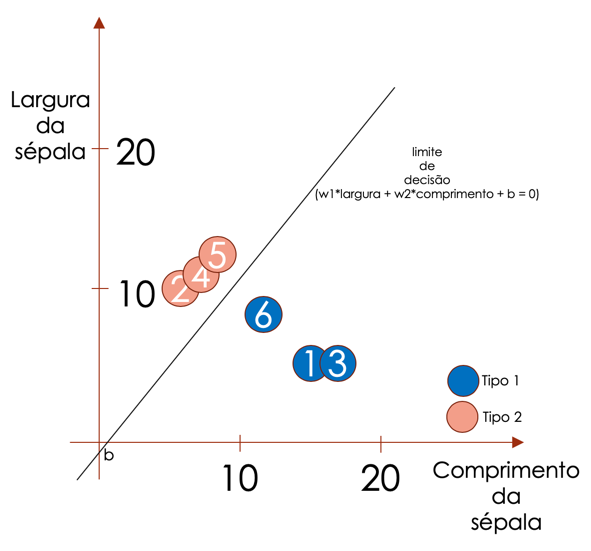
\includegraphics[width=300pt]{figuras/classes_linearmente_separaveis.png}
  \caption{Classes linearmente separáveis}
  \label{fig:classes_separadas}
\end{figure}

Embora apenas nos últimos anos a sociedade tenha absorvido o conceito de aprendizado de máquina, é importante ressaltar que seus princípios foram originados entre os anos de 1943 e 1958, nos quais vários pesquisadores ganharam destaque por contribuições pioneiras como:
\begin{itemize}
    \itemsep-1em
    \item Warren McCulloch e Walter Pitts
    (\citeyear{mcculloch1943logical}) por introduzirem a ideia de redes neurais como máquinas de computação.
    \item Donald Hebb (\citeyear{hebb1949organization}) que postulou a primeira regra de aprendizado auto-organizável.
    \item Frank Rosenblatt (\citeyear{rosenblatt1958two}) que criou um dispositivo eletrônico, de acordo com os princípios biológicos, capaz de aprender de forma supervisionada.
\end{itemize}

O perceptron simples, cria um hiperplano definido pela equação abaixo que separa duas regiões num espaço que abrange $m$ dimensões:
\begin{equation*}
    \sum_{i=1}^{m} w_i * x_i + b = 0
\end{equation*}

Conforme apresentado na figura \ref{fig:perceptron}, os pesos sinápticos do Preceptron são dados por $w_1, w_2, w_3...$. De forma correspondente, as entradas aplicadas ao perceptron são denotadas por $x_1, x_2, x_3...$

\begin{figure}[H]
  \centering
  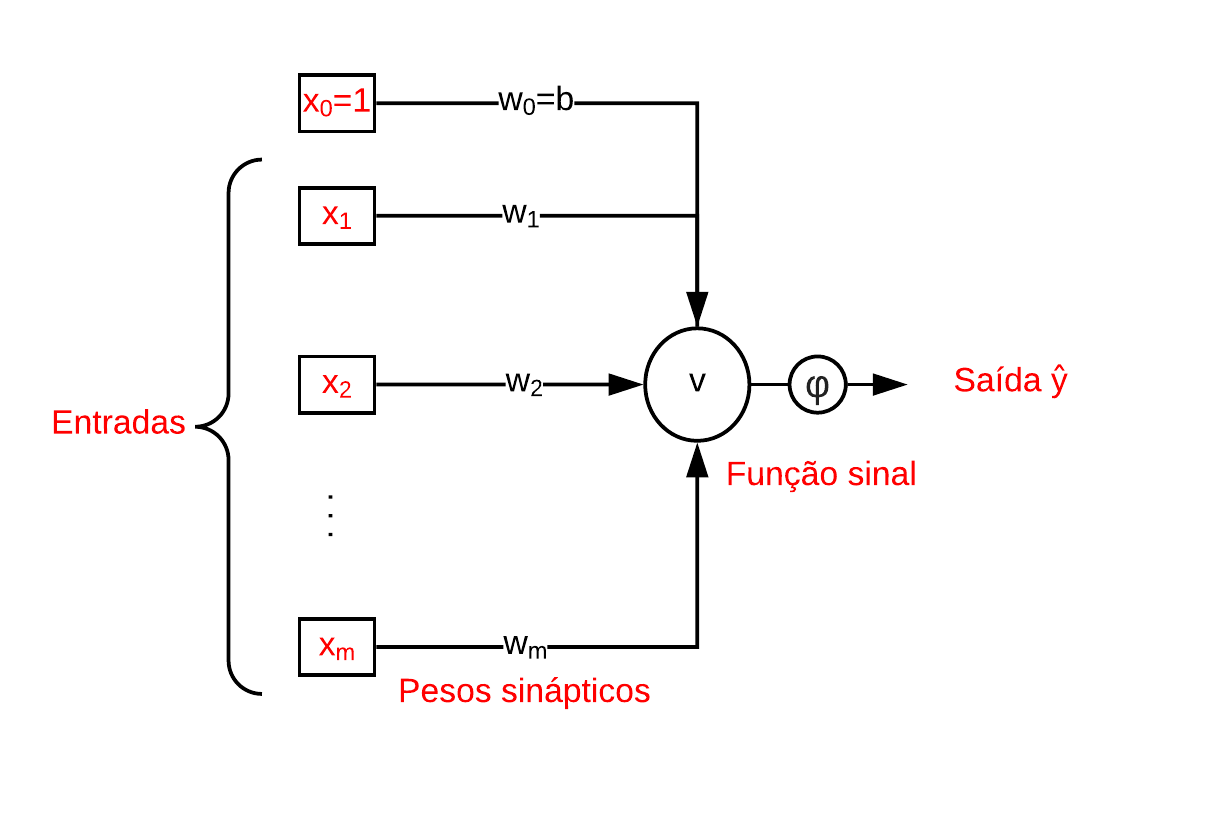
\includegraphics[width=300pt]{figuras/Perceptron.png}
  \caption{Perceptron}
  \label{fig:perceptron}
\end{figure}

Já a função sinal $\phi$ (função de ativação) classifica como 1 (classe 1) se o resultado da combinação linear das entradas pelos seus pesos ($v$) for positivo. Caso contrário, o limitador classifica como -1 (classe 2).

Assumindo que $x$ é o vetor com dimensões $m+1$ por $1$, sendo que o primeiro elemento tem o valor fixo de $+1$ e assumindo que $w$ é vetor de pesos com dimensões $m+1$ por $1$, sendo que o primeiro elemento é igual ao bias $b$, temos que cada computação/iteração $n$ aplica o seguinte ajuste ao vetor de pesos:

\begin{equation*}
\label{eqn:ajustePesoNeuronio}
    w_{n + 1}=w_n + \eta * [d_n - \hat{y}_n] * x_n
\end{equation*}

A maioria algoritmos de aprendizado de máquina tem hiperparâmetros que são variáveis cujos valores são determinados antes do início do treinamento. No caso do Perceptron, o hiperparâmetro taxa de aprendizado $\eta$ indica a intensidade do ajuste aplicado ao vetor de peso na iteração $n$. A convergência da rede neural na separação das classes é garantida independente do valor de $\eta$, mas uma alta taxa de aprendizado resultará num aprendizado mais rápido. É necessário porém, que $0<\eta<=1$ sendo que, de acordo com Lippmann (\citeyear{lippmann1987}), os seguintes conflitos devem ser considerados para a escolha do valor de $\eta$:

\begin{itemize}
    \item Considerar as entradas passadas com mais relevância para prover pesos estáveis, o qual requer um valor pequeno de $\eta$
    \item Rápida apdaptação com respeito às mudanças reais nas distribuições do processo responsável pela geração do vetor de entrada $x$, o qual requer um valor alto para $\eta$ 
\end{itemize}

O modelo Perceptron foi criticado por Minsky e Selfridge (\citeyear{minsky1961steps}) que apontaram que o Perceptron definido por Rosenblatt, mesmo com múltiplas camadas, não poderia nem mesmo generalizar a noção de paridade binária, quanto mais fazer abstrações gerais.
Essa afirmação colocou em cheque o que acreditava-se ser possível com redes neurais até meados de 1980.

No entanto, a conjuctura feita por Minsky e Papert (\citeyear{minsky1969perceptron}) pareceu irrelevante uma vez que modelos mais avançados de redes neurais surgiram. Dentre eles: perceptrons de múltiplas camadas (MLP) com algoritmo de retro-propagação, redes função de base radial (RBF) e máquina de suporte de vetores (SVM). Na seção \ref{sec:redeneuralmlp} a MLP será explicada com mais detalhes.

\section{Rede Neural Artificial Perceptron Múltiplas Camadas}
\label{sec:redeneuralmlp}
Frank Rosenblatt propôs em 1958 o modelo Perceptron que era composto de uma estrutura de rede de neurônios e uma regra de aprendizado. Esse modelo possuía apenas uma camada e tinha como saída um valor
binário. Entretanto, por possuir uma única camada, este modelo podia ser aplicado apenas a problemas linearmente separáveis.
Essa limitação foi resolvida com a criação e aplicação do algoritmo back-propagation (\citeyear{rumelhart1986parallel}) nas redes de múltiplas camadas ou Multi Layer Perceptron (MLP). 

\begin{figure}[H]
    \centering
  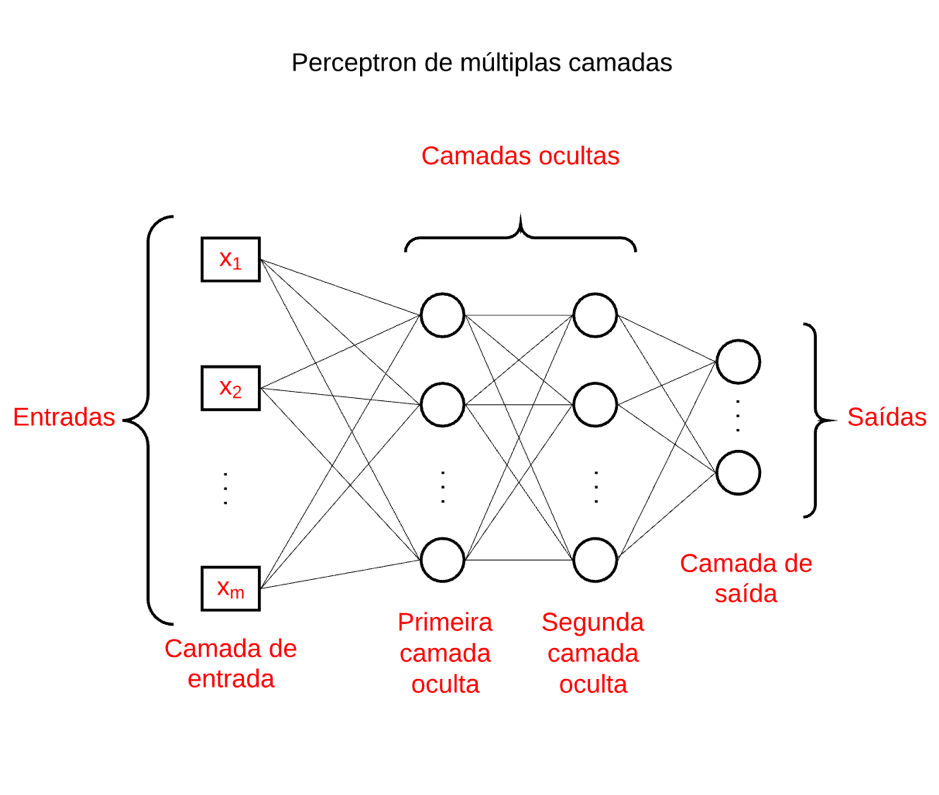
\includegraphics[width=350pt]{figuras/MLP.png}
  \caption{MLP}
  \label{fig:MLP}
\end{figure}

Acima está ilustrada uma arquitetura de rede neural na qual podem ser identificadas a camada de entrada, as camadas ocultas e a camada de saída. Tanto a camada de entrada quanto a camada de saída pode ser uni ou multivalorada. Essa figura representa o primeiro modelo de redes de múltiplas camadas capaz de resolver problemas não linearmente separáveis.

A MLP é uma rede neural estruturada da seguinte forma:
\begin{itemize}
    \item Cada neurônio (Perceptron) possui uma função de ativação não linear que é diferenciável
    \item A rede contém uma ou mais camadas que são \textit{ocultas} dos nós de entrada e dos nós de saída
    \item A rede possui um alto grau de conectividade cuja extensão é determinada pelos pesos sinápticos da rede
\end{itemize}

As limitações do Perceptron foram, depois de muito tempo, sucumbidas com essa nova estrutura. Porém essas características acarretaram na dificuldade de interpretação do comportamento da rede.
% DESENVOLVER MAIS

Foi em meados de 1985 que o termo ``back propagation'' se popularizou com a publicação do livro ``Parallel Distributed Processing'' (Rumelhart e McClelland) o que também trouxe otimismo sobre o processo de aprendizado nos perceptrons de múltiplas camada, pois a partir de então o processamento paralelo foi possível.

Esta conectividade é definida pelos pesos sinápticos. Uma camada é suficiente para aproximar qualquer função contínua e duas
camadas podem aproximar qualquer função matemática \cite{cybenko1989approximation}.


Como mencionado acima, o algoritmo de retro-propagação foi o que possibilitou a rede neural a resolver problemas não linearmente separáveis. As duas fases deste algoritmo serão explanadas abaixo:

\begin{itemize}
    \item Na fase de \textit{propagação}, os pesos sinápticos da rede são fixados e o sinal da entrada é propagado através da rede, camada a camada, até que alcance a saída.
    \item Na fase de retro-propagação, um sinal de erro é produzido ao se comparar a saída da rede neural ($\hat{y}$) com a resposta desejada ($y$). Este sinal é então propagado na rede, camada a camada, mas na direção reversa. Os pesos sinápticos são ajustados tanto na camada de saída quanto nas camadas ocultas.
\end{itemize}

\begin{figure}[H]
    \centering
  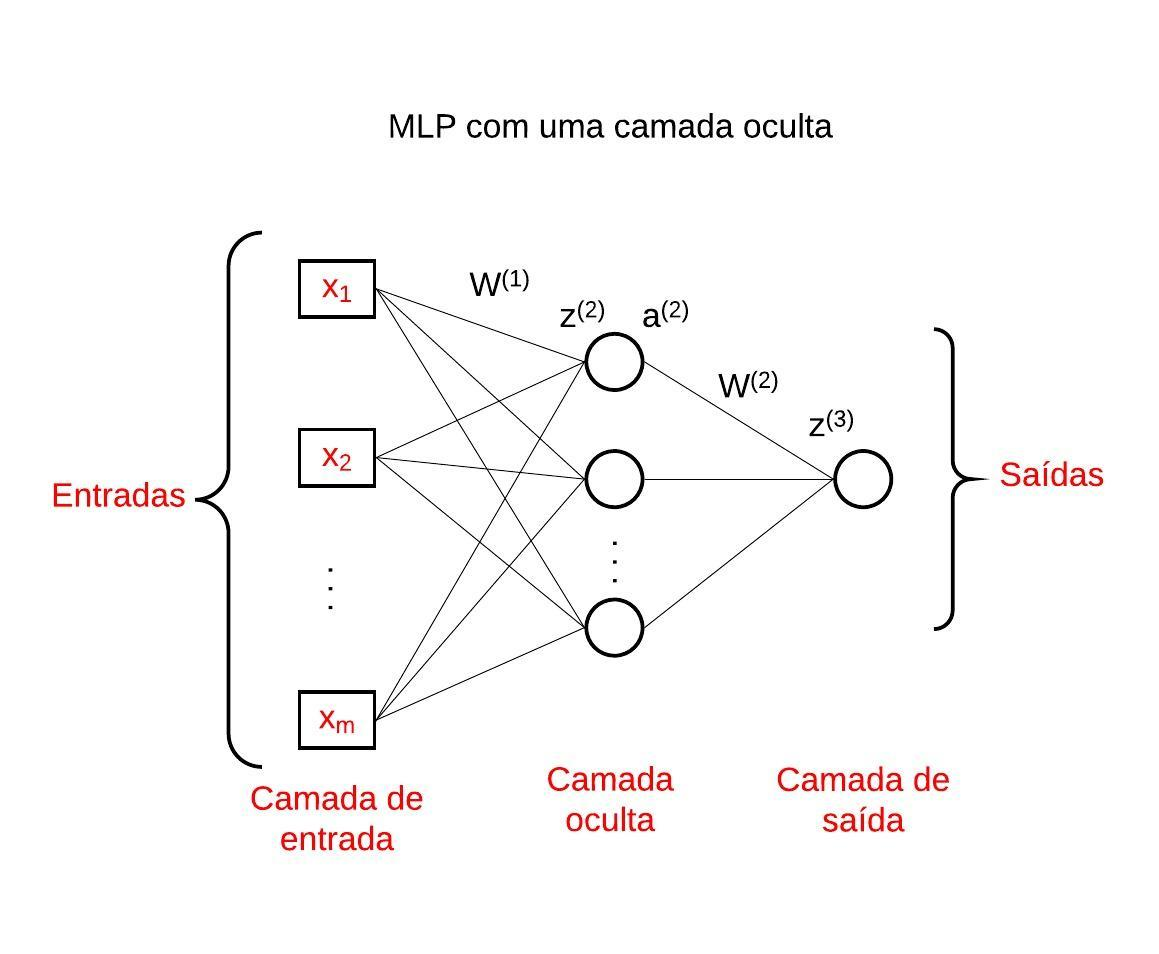
\includegraphics[width=350pt]{figuras/MLP_uma_camada.jpeg}
  \caption{MLP uma camada}
  \label{fig:MLP uma camada}
\end{figure}

A MLP \ref{fig:MLP uma camada} ilustrada acima tem uma camada de entrada, uma camada oculta e uma camada de saída. Abaixo será apresentado como ela irá predizer $\hat{y}$, e como este será aos poucos ser cada vez mais parecido com a resposta desejada $y$ depois de alguns ajustes de pesos sinápticos regrados pelas funções de custo de acordo com os vetores de pesos sinápticos $W^{(1)}$ e $W^{(2)}$ que minimizam a diferença entre $\hat{y}$ e $y$.

% Dado que $X_{r,c} = $ 
% $
%  \begin{pmatrix}
%   x_{1,1} & x_{1,2} & \cdots & x_{1,c} \\
%   x_{2,1} & x_{2,2} & \cdots & x_{2,c} \\
%   \vdots  & \vdots  & \ddots & \vdots  \\
%   x_{r,1} & x_{r,2} & \cdots & x_{r,c} 
%  \end{pmatrix}
% % \end{equation}
% $, que $y_{r} = $
% $
%  \begin{pmatrix}
%  y_{1} \\
%  y_{2} \\
%  \vdots  \\
%  y_{r}
%  \end{pmatrix}
% $
% e que $W_{r,c} = $
% $
% \begin{pmatrix}
%   w_{1,1} & w_{1,2} & \cdots & w_{1,c} \\
%   w_{2,1} & w_{2,2} & \cdots & w_{2,c} \\
%   \vdots  & \vdots  & \ddots & \vdots  \\
%   w_{r,1} & w_{r,2} & \cdots & w_{r,c}
% \end{pmatrix}
% $. 

Assumindo que $X = [x_1, x_2,...x_m]$ e que $W^{(1)}$ corresponde aos pesos sinápticos da primeira camada, tem-se que a ativação da segunda camada é dada por 

\begin{equation}
z^{(2)} = XW^{(1)}
\end{equation}

É necessário aplicar a função de ativação a cada valor de $z^{(2)}$, portanto tem-se que
\begin{equation}
a^{(2)} = f(z{(2)})
\end{equation}

Para finalizar a fase de propagação, é necessário propagar $a^{(2)}$ até o nó de saída da rede neural. Portanto, tem-se que a ativação da camanda de saída é dada por
\begin{equation}
z^{(3)} = a^{(2)}W^{(2)}
\end{equation}

Novamente é necessário aplicar a função de ativação a cada valor de $z^{(3)}$. Finalmente tem-se que $\hat{y}$ é dado por
\begin{equation}
\hat{y} = f(z^{(3)})
\end{equation}

Com isso, tem-se que o valor de saída da rede. Porém faz-se necessário determinar o quão certo ou errado a saída da rede $y$ é similar ao valor esperado $d$, ou seja, determina-se o custo.

\section{Função de custo}

O algoritmo de retropropagação procura encontrar pesos $w$ e biases $b$ de forma que a saída da rede neural $y$ se aproxime de todas as entradas $x$. Para quantificar o quão bem este objetivo está sendo alcançado, usa-se a função de custo, também conhecida por \textit{erro} ou \textit{função objetivo} representada pela equação abaixo:

\begin{equation}
\label{funcaodecusto}
C(w,b) = \sum_{i=1}^{r} \frac{1}{2}(y_i - \hat{y_i})^2    
\end{equation}

Neste caso, a função de custo quadrática, também conhecida como erro médio quadrático (MSE) é uma função positiva uma vez que todo termo somado é positivo. Além disso, o custo $C(w,b)$ se aproxima de zero quando $\hat{y}$ se aproxima de $y$. Portanto o algoritmo fez um bom trabalho se pôde encontrar pesos e biases de forma que $C(w,b) \approx 0$. O objetivo do algoritmo então é minimizar o custo em função dos pesos e biases.

% O custo é uma função de duas coisas: as entradas e os pesos. Como sabemos, não é possível alterar os dados de entrada, porém é possível alterar os pesos de forma que a função de custo seja minimizada, ou seja, procura-se uma combinação ótima dos valores de $W$ que resultem em um $J$ próximo ou igual a zero.

Quanto mais combinações tiverem que ser testadas, mais tempo computacional será necessário para encontrar a combinação ótima de $W$ que resulte num menor valor para a função de custo.

Usa-se a derivada parcial para determinar a taxa de variação de cada valor de $W^{(1)}$ em relação a função de custo. 

% O uso desta técnica para cada entrada da rede neural, indica em qual direção do plano formado pelas diferentes dimensões $w$ minimiza a função de custo em relação a $W^{(1)}$:

% \begin{equation}
% \dfrac{\partial J}{\partial W^{(1)}} = 
% \begin{pmatrix}
%   \dfrac{\partial J}{\partial w^{(1)}_{1,1}} & \dfrac{\partial J}{\partial w^{(1)}_{1,2}} & \cdots & \dfrac{\partial J}{\partial w^{(1)}_{1,c}} \\
%   \dfrac{\partial J}{\partial w^{(1)}_{2,1}} & \dfrac{\partial J}{\partial w^{(1)}_{2,2}} & \cdots & \dfrac{\partial J}{\partial w^{(1)}_{2,c}} \\
%   \vdots  & \vdots  & \ddots & \vdots  \\
%   \dfrac{\partial J}{\partial w^{(1)}_{r,1}} & \dfrac{\partial J}{\partial w^{(1)}_{r,2}} & \cdots & \dfrac{\partial J}{\partial w^{(1)}_{r,c}} \\
% \end{pmatrix}
% \end{equation}

% Já a função de custo de $W^{(2)}$ é dada por: 
% \begin{equation}
% \dfrac{\partial J}{\partial W^{(2)}} = 
% \begin{pmatrix}
%   \dfrac{\partial J}{\partial w^{(2)}_{1,1}} \\
%   \dfrac{\partial J}{\partial w^{(2)}_{2,1}} \\
%   \vdots \\
%   \dfrac{\partial J}{\partial w^{(2)}_{c,1}}
% \end{pmatrix}
% \end{equation}

% onde $c$ é o número de neurônios na camada oculta e $r$ é o número de entradas do conjunto de treinamento.

\begin{equation}
custo = \sum_{i=1}^{r} \frac{1}{2}(y_i - f(f(XW^{(1)})W^{(2)})^2    
\end{equation}

Deriva-se os dois lados da equação, assim tem-se:

\begin{equation}
    \frac{\partial J}{\partial W^{(2)}} = \partial \sum_{i=1}^{r} \frac{ \frac{1}{2}(y_i - \hat{y_i})^2}{\partial W^{(2)}}
\end{equation}

Como a soma das derivadas é o mesmo que a derivada das somas, é possível mover o somatório conforme segue:

\begin{equation}
    \frac{\partial J}{\partial W^{(2)}} = \sum_{i=1}^{r} \frac{\partial \frac{1}{2}(y_i - \hat{y_i})^2}{\partial W^{(2)}}
\end{equation}

Se considerado apenas o primeiro exemplar do conjunto de treinamento, ou seja, se consideramos apenas a primeira linha da matriz $X$, é possível omitir o somátório e adicionar cada um dos termos derivados depois:

\begin{equation}
    \frac{\partial J}{\partial W^{(2)}} = \frac{\partial \frac{1}{2}(y_i - \hat{y_i})^2}{\partial W^{(2)}}
\end{equation}

Por conta da regra da potenciação de derivada, tem-se:

\begin{equation}
    \frac{\partial J}{\partial W^{(2)}} = (y - \hat{y})
\end{equation}

Resta agora derivar a função $(y-\hat{y})$ em relação a $W^{(2)}$. 

O gráfico abaixo apresenta de maneira simplificada a rede neural com apenas um nó em cada camada.



% \begin{figure}[h]
%   \begin{tikzpicture}
%     %%Create a style for the arrows we are using
%     \tikzset{normal arrow/.style={draw,-triangle 45,very thick}}
%     %%Create the different coordinates to place the nodes
%     \path (0,0) coordinate (1) ++(0,-2) coordinate (2) ++(0,-2) coordinate (3);
%     \path (1) ++(-3,-.2) coordinate (x1);
%     \path (3) ++(-3, .2) coordinate (x2);
%     %%Use the calc library and partway modifiers to generate the second and third level points
%     \path ($(1)!.5!(2)!3 cm!90:(2)$) coordinate (4);
%     \path ($(2)!.5!(3)!3 cm!90:(3)$) coordinate (5);
%     \path ($(4)!.5!(5)!3 cm!90:(5)$) coordinate (6);
%     \path (6) ++(3,0) coordinate (7);
%     %%Place nodes at each point using the foreach construct
%     \foreach \i/\color in {1/Magenta!60,2/MidnightBlue!60,3/CadetBlue!80,4/CadetBlue!80,5/CadetBlue!80,6/CadetBlue!80}{
%       \node[draw,circle,shading=axis,top color=\color, bottom color=\color!black,shading angle=45] (n\i) at (\i) {$f_{\i}(e)$};
%     }
%     %%Place the remaining nodes separately
%     \node (nx1) at (x1) {$\mathbf{x_1}$};
%     \node (nx2) at (x2) {$\mathbf{x_2}$};
%     \node (ny)  at (7)  {$\mathbf{y}$};
%     %%Drawing the arrows
%     \path[normal arrow] (nx1) -- (n1);
%     \path[normal arrow] (nx1) -- (n3);
%     \path[normal arrow] (nx2) -- (n1);
%     \path[normal arrow] (nx2) -- (n3);
%     \path[normal arrow] (n1)  -- (n4);
%     \path[normal arrow] (n1)  -- (n5);
%     \path[normal arrow] (n2)  -- (n4);
%     \path[normal arrow] (n2)  -- (n5);
%     \path[normal arrow] (n3)  -- (n4);
%     \path[normal arrow] (n3)  -- (n5);
%     \path[normal arrow] (n4)  -- (n6);
%     \path[normal arrow] (n5)  -- (n6);
%     \path[normal arrow] (n6)  -- (ny);
%     %%Drawing the cyan arrows including the labels
%     \path[normal arrow,Cyan] (nx1) -- node[above=.5em,Cyan] {$\mathbf{w_{(x1)2}}$} (n2);
%     \path[normal arrow,Cyan] (nx2) -- node[below=.5em,Cyan] {$\mathbf{w_{(x2)2}}$} (n2);
%   \end{tikzpicture}
% \caption{Do not forget!
% Make it explicit enough that readers
% can figure out what you are doing.}
% \end{figure}

\begin{figure}[H]
    \centering
  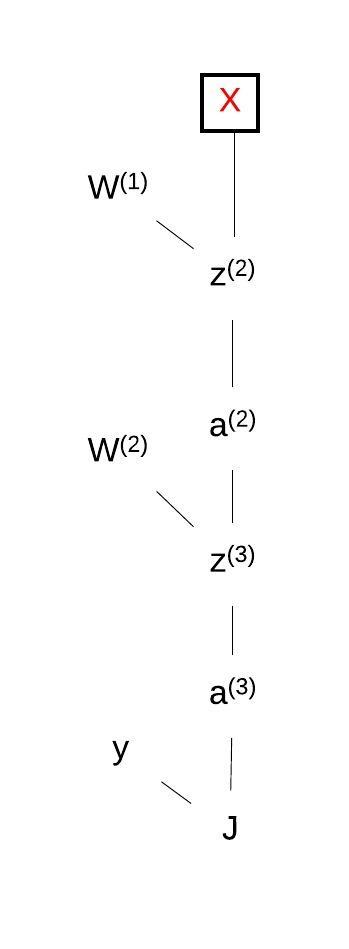
\includegraphics[width=100pt]{figuras/derivadas_parciais_um_no_por_camada.jpeg}
  \caption{Cálculo do custo}
  \label{fig:derivadas_parciais_um_no_por_camada}
\end{figure}

Assumindo que $a^{(3)}$ no gráfico acima representa $\hat{y}$ e aplicando a da regra da cadeia a fim determinar a \textit{sensibilidade} de $W^{(2)}$ em relação ao custo , tem-se:

\begin{equation}
    \frac{\partial J}{\partial W^{(2)}} = (y - \hat{y})(-\frac{\partial \hat{y}}{\partial z^{(3)}})
\end{equation}

Sabendo que $\hat{y}=f(z^{(3)})$, tem-se:
\begin{equation}
    \frac{\partial J}{\partial W^{(2)}} = -(y - \hat{y})\frac{\partial \hat{y}}{\partial z^{(3)}}\frac{\partial z^{(3)}}{\partial W^{(2)}}
\end{equation}

$\frac{\partial \hat{y}}{\partial z^{(3)}}$ representa aqui a derivada da função de ativação, portanto será representada por $f'(z^{(3)})$ como mostrado abaixo:
\begin{equation}
    \frac{\partial J}{\partial W^{(2)}} = -(y - \hat{y}) f'(z^{(3)}) \frac{\partial z^{(3)}}{\partial W^{(2)}}
\end{equation}

Sabendo que $z^{(3)}=a^{(2)}W^{(2)}$, temos que $a^{(2)}$, é a taxa de variação de $z^{(3)}$ em relação a $W^{(3)}$.

$-(y-\hat{y})$ representa a seguinte matriz:

\begin{equation*}
\begin{pmatrix}
  -y_1 - \hat{y}_1\\
  -y_2 - \hat{y}_2\\
  \vdots \\
  -y_r - \hat{y}_r
\end{pmatrix}
\end{equation*}

Já $f'(z^{(3)})$ representa a seguinte matriz:

\begin{equation*}
\begin{pmatrix}
  f'(z^{(3)}_1)\\
  f'(z^{(3)}_2)\\
  \vdots \\
  f'(z^{(3)}_r)
\end{pmatrix}
\end{equation*}

A multiplicação destas matriz resulta noutra matriz $\delta^{(3)}$ conforme segue:

\begin{equation*}
\begin{pmatrix}
  \delta_1^{(3)}\\
  \delta_2^{(3)}\\
  \vdots \\
  \delta_r^{(3)}
\end{pmatrix}
\end{equation*}

A equação $ z^{(3)} = a^{(2)} W^{(2)} $ representa a ativação da segunda camada que é dada por $(a^{(2)})^T$, portanto tem-se que que o custo da terceira camada é dado por:

\begin{equation}
    \frac{\partial J}{\partial W^{(2)}} = (a^{(2)})^T \delta^{(3)}
\end{equation}

O mesmo processo é feito para se determinar o custo da primeira camada, portanto tem-se:

\begin{equation}
    \frac{\partial J}{\partial W^{(1)}} = \delta^{(3)} \frac{\partial z^{(3)}}{\partial a^{(2)}} \frac{\partial a^{(2)}}{\partial W^{(1)}}
\end{equation}

\begin{equation}
    \frac{\partial J}{\partial W^{(1)}} = \delta^{(3)} \frac{\partial z^{(3)}}{\partial a^{(2)}} \frac{\partial a^{(2)}}{\partial z^{(2)}} \frac{\partial z^{(2)}}{\partial W^{(1)}}
\end{equation}

Fazendo as devidas substituições:
\begin{equation}
    \frac{\partial J}{\partial W^{(1)}} = \delta^{(3)} (W^{(2)})^T f'(z^{(2)}) \frac{\partial z^{(2)}}{\partial W^{(1)}}
\end{equation}

Finalmente, usando a transposta da matriz X, tem-se a seguinte equação que representa o custo da primeira camada:
\begin{equation}
    \frac{\partial J}{\partial W^{(1)}} = X^T \delta^{(3)} (W^{(2)})^T f'(z^{(2)})
\end{equation}

Resumindo, tem-se que a correção $\Delta w_{ij}(n)$ aplicada ao peso da conexão sináptica do neurônio $i$ da camada $j$ é definida por:

\begin{equation*}
    \begin{pmatrix} 
    \text{Correção do peso} \\
    \Delta w_{ij}(n)
    \end{pmatrix}
    =
    \begin{pmatrix} 
    \text{taxa de aprendizado} \\ 
    \eta
    \end{pmatrix}
    \times
    \begin{pmatrix} 
    \text{gradiente local} \\ 
    \delta_j(n)
    \end{pmatrix}
    \times
    \begin{pmatrix} 
    \text{entrada do neurônio $j$} \\ 
    $y$_i(n)
    \end{pmatrix}
\end{equation*}

O grandiente local $\delta_j(n)$ depende se o neurônio $j$ é oculto ou de saída:
\begin{enumerate}
    \item Se o neurônio $j$ for de saída, $\delta_j(n)$ é igual ao produto da derivada $\phi_j'(v_j(n))$ pelo erro $e_j(n)$ no neurônio $j$;
    \begin{equation*}
        \delta_j(n) = e_j(n)\phi'_j(v_j(n))
    \end{equation*}
    \item Se o neurônio $j$ for oculto, $\delta_j(n)$ é igual ao produto da derivada $\phi_j'(v_j(n))$ pelas somas ponderadas de $\delta$ calculado para o neurônio na próxima camada que está conectado ao neurorio $j$.
    \begin{equation*}
        \delta_j(n) = \phi'_j(v_j(n)) \sum_k \delta_k(n)w_{kj}(n)
    \end{equation*}
\end{enumerate}

\subsection{Funções de ativação}

Nesta seção será apresentado porque é conveniente usar funções do tipo sigmoid em redes de múltiplas camadas.
O cálculo de $\delta$ para cada neurônio $j$ requer a derivada da função $\phi$ associada aquele neurônio. O único requisito para que a derivada desta função exista, é que a função seja contínua.
Um exemplo de função contínua não linear é a sigmoid (nome proveniente de sigma que é a letra s do alfabeto grego por conta do formato apresentado quando esta função é plotada.
Duas formas de sigmoid são apresentadas abaixo:

\begin{enumerate}
    \item Função logística:
    \begin{figure}[H]
    \centering
    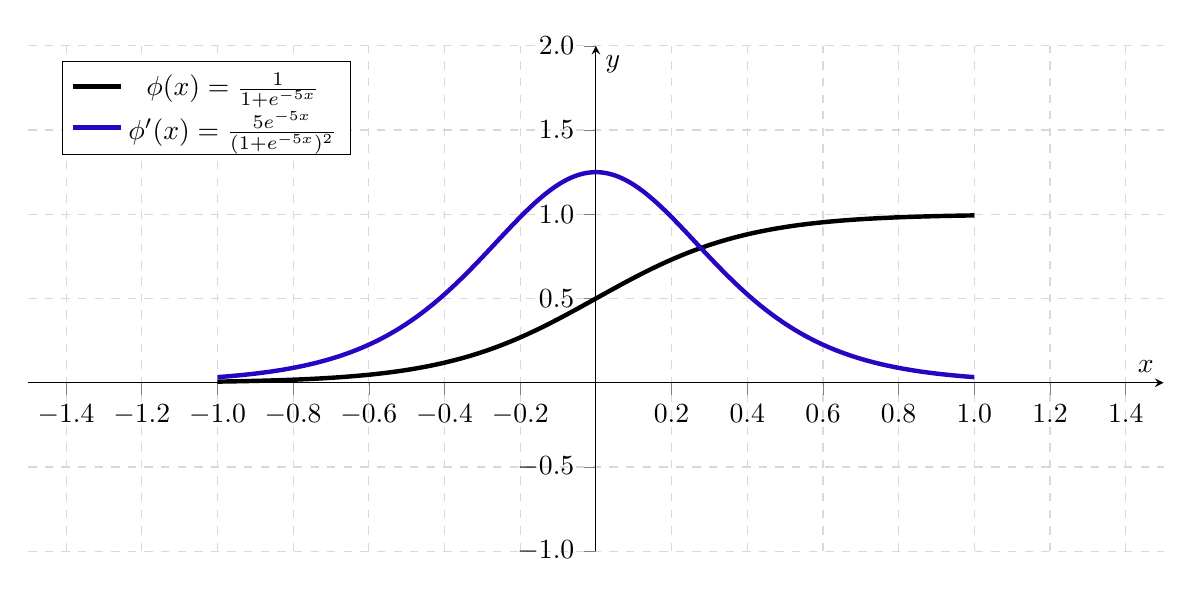
\begin{tikzpicture}
    \begin{axis}[
    	legend pos=north west,
        axis x line=middle,
        axis y line=middle,
        x tick label style={/pgf/number format/fixed,
                            /pgf/number format/fixed zerofill,
                            /pgf/number format/precision=1},
        y tick label style={/pgf/number format/fixed,
                            /pgf/number format/fixed zerofill,
                            /pgf/number format/precision=1},
        grid = major,
        width=16cm,
        height=8cm,
        grid style={dashed, gray!30},
        xmin=-1.5, xmax= 1.5,
        ymin= -1, ymax= 2,
        domain=-1:1,
        %axis background/.style={fill=white},
        xlabel=$x$,
        ylabel=$y$,
        tick align=outside,
        enlargelimits=false]
      % plot the stirling-formulae
      \addplot[ultra thick,samples=500] {1/(1+exp(-5*x))};
      \addplot[blue, ultra thick, samples=500]{(5*exp(-5*x))/((exp(-5*x)+1)*(exp(-5*x)+1))};
      \addlegendentry{$\phi(x)=\frac{1}{1+e^{-5x}}$}
      \addlegendentry{$\phi'(x)=\frac{5e^{-5x}}{(1+e^{-5x})^2}$}
    \end{axis}
    \end{tikzpicture}
    \caption{Gráfico da função logística e sua derivada}
    \end{figure}
    \begin{equation}
        \phi(x) = \frac{1}{1+e^{-\alpha x}}, \: com \: \alpha > 0
    \end{equation}
    Diferenciando esta função em relação a $x$, tem-se:
    \begin{equation}
        \frac{\partial \phi(x)}{\partial x} = \frac{\partial (1+e^{-\alpha x})^{-1}}{\partial x}
    \end{equation}
    Resolvendo a equação de acordo com a regra da potência de derivada, tem-se:
    \begin{equation}
        \frac{\partial \phi(x)}{\partial x} = (1+e^{-\alpha x})^{-2} (e^{-\alpha x}) \alpha
    \end{equation}
    Reescrevendo a equação acima, tem-se:
    \begin{equation}
        \frac{\partial \phi(x)}{\partial x} = \left(\frac{1}{1+e^{-\alpha x}}\right) \left(\frac{e^{-\alpha x}}{1+e^{-\alpha x}} \right) \alpha
    \end{equation}
    Adicionando e subtraindo 1 do numerador da segunda parcela da equação, tem-se:
    \begin{equation}
        \frac{\partial \phi(x)}{\partial x} = \left(\frac{1}{1+e^{-\alpha x}}\right) \left(\frac{\textbf{1}+e^{-\alpha x} - \textbf{1}}{1+e^{-\alpha x}}\right) \alpha
    \end{equation}
    Expandindo a equação acima, tem-se:
    \begin{equation}
        \frac{\partial \phi(x)}{\partial x} = \left(\frac{1}{1+e^{-\alpha x}}\right) \left(\frac{1+e^{-\alpha x}}{1+e^{-\alpha x}} - \frac{1}{1+e^{-\alpha x}}\right) \alpha
    \end{equation}
    Lembrando que $\frac{1}{1+e^{-\alpha x}} = \phi(x)$ e fazendo as devidas substituições, tem-se:
    \begin{equation}
        \frac{\partial \phi(x)}{\partial x} = \phi(x) (1- \phi(x)) \alpha
    \end{equation}
    Essa simplificação permite que o cálculo do gradiente local para qualquer neurônio $j$ seja dado por:
        \begin{itemize}
        \item Para neurônios da camada de saída:
        \begin{equation}
            \begin{split}
            \delta_j(n) = e_j(n)\phi'(v_j(n)) \\
            \delta_j(n) = \alpha[y_j(n) - \hat{y_j}(n)]\hat{y_j}(n)[1 - \hat{y_j}(n)]    
            \end{split}
        \end{equation}
        \item Para neurônios da camada oculta:
        \begin{equation}
            \begin{split}
            \delta_j(n) = \phi'(v_j(n)) \sum_k \delta_k(n)w_{kj}(n) \\
            \delta_j(n) = \alpha y_j(n)[1 - y_j(n)]\sum_k \delta_k(n)w_{kj}(n)
            \end{split}
        \end{equation}
    \end{itemize}
Percebe-se que a função $\phi'(x)=x*(1-x)$, em azul, tem máximo em 0.5 e mínimos em 0 e 1.0. Considerando que o ajuste num peso sináptico é proporcional a derivada $\phi_j(v_j(n))$, os pesos que têm mais influência no ajuste, são aqueles que têm ativação nos seus intervalos intermediários. De acordo com David Rumelhart (\citeyear{rumelhart1986parallel}), é essa característica do algoritmo de retro-propagação que contribui para sua estabilidade como algoritmo de aprendizado.
\item Função tangente hiperbólica
    \begin{figure}[H]
    \centering
    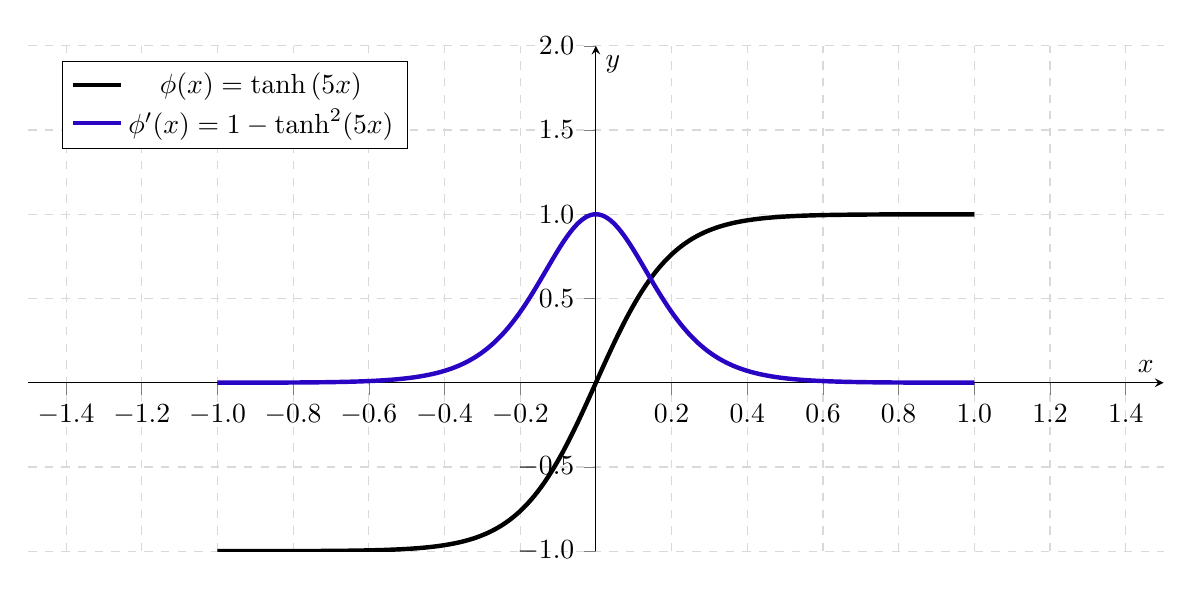
\begin{tikzpicture}
    \begin{axis}[
    	legend pos=north west,
        axis x line=middle,
        axis y line=middle,
        x tick label style={/pgf/number format/fixed,
                            /pgf/number format/fixed zerofill,
                            /pgf/number format/precision=1},
        y tick label style={/pgf/number format/fixed,
                            /pgf/number format/fixed zerofill,
                            /pgf/number format/precision=1},
        grid = major,
        width=16cm,
        height=8cm,
        grid style={dashed, gray!30},
        xmin=-1.5, xmax= 1.5,
        ymin= -1, ymax= 2,
        domain=-1:1,
        %axis background/.style={fill=white},
        xlabel=$x$,
        ylabel=$y$,
        tick align=outside,
        enlargelimits=false]
      % plot the stirling-formulae
    \addplot[ultra thick,samples=500] {tanh(5* \x)};
      \addplot[blue, ultra thick, samples=500]{1-((tanh(5* \x) * (tanh(5* \x)))};
    %   \addplot[yellow, ultra thick, samples=500]{5[}
      \addlegendentry{$\phi(x)=\tanh{(5x)}$}
      \addlegendentry{$\phi'(x)= 1 - \tanh^2(5x)$}
    \end{axis}
    \end{tikzpicture}
    \caption{Gráfico da função tangente hiperbólica e sua derivada}
    \end{figure}
Outra forma de função sigmoid é a tangente hiperbólica, cuja equação mais geral é dada por:

\begin{equation}
    \phi(x)=a*tanh(b*x)
\end{equation}

onde a e b são constantes positivas. Na verdade, esta função é função logística re-escalada e tendenciosa.
Sua derivada em relação a $x$ é dada por:
\begin{equation}
    \begin{split}
    \phi'(x)=ab(sech^2(bx) \\
    \phi'(x)=ab(1-tanh^2(bx) \\
    \phi'(x)=\frac{b}{a}[a-x][a+x]
    \end{split}
\end{equation}
\begin{itemize}
    \item Para um neurônio $j$ na camada de saída, tem-se:
        \begin{equation}
            \begin{split}
                \delta_j(n)=e_j(n)\phi'(v_j(n)) \\
                \delta_j(n)=\frac{b}{a}[y_j(n)-\hat{y}_(n)][a-\hat{y}_(n)][a+\hat{y}_(n)]
            \end{split}
        \end{equation}
    \item Para um neurônio $j$ na camada oculta, tem-se:
    \begin{equation}
        \begin{split}
        \delta_j(n) = \phi'(v_j(n)) \sum_k \delta_k(n)w_{kj}(n) \\
        \delta_j(n) = \frac{b}{a}[a-y_j(n)][a+y_j(n)] \sum_k \delta_k(n)w_{kj}(n)
        \end{split}
    \end{equation}
\end{itemize}
\end{enumerate}

\subsection{Taxa de aprendizado e constante momentum}

O perceptron de múltiplas camadas aprende ao passo que ajusta os pesos de acordo com a função de custo. A velocidade com que se dá o aprendizado depende de algums fatores como valor inicial de cada peso, escala de cada atributo de entrada, taxa de aprendizado e constante momentum. Nesta seção será explicado como a taxa de aprendizado e o valor do momemtum afetam a velocidade do aprendizado da rede e o que deve ser considerado para determinar seus valores.

O algoritmo de retro propagação procura encontrar os valores dos pesos sinápticos que minimizam a função de custo. Para isso, usa-se o gradiente descendente que como foi explicado em seções acima, é dado pela derivada do custo em relação aos pesos. Segue uma forma lúdica de como o algoritmo faz isso: Imagine que você está numa montanha com muita névoa e que seu objetivo é descer antes do pôr do sol.
Você decide olhar em volta e ir para o ponto mais baixo ao seu redor, porém há tanta névoa que você não enxerga. Por sorte, você tem um aparelho  que mensura a inclinação. Você aponta o aparelho para chão num ponto próximo a você e compara com as medições a sua volta.
Você anda para o ponto mais baixo. Se você repetir esse processo, eventualmente chegará na base da montanha. Mas tem um problema, a medição com o aparelho leva um tempo. Então seu objetivo é usar menos o aparelho para que alcance a base da montanha antes do pôr do sol. 
Você representa o algoritmo. 

A montanha representa a função de custo. A base da montanha representa o mínimo global. A inclinação medida pelo aparelho representa a inclinação da superfície de erro naquele ponto. O aparelho usado para medir a inclinação é a derivada do função de erro quadrado naquele ponto. A direção escolhida para descer está alinhada com o gradiente da superfície de erro naquele ponto. O tempo que leva para descer até o ponto mais baixo local é a taxa de aprendizado.
Quanto menor o valor da taxa de aprendizado, mais suave é a trajetória na superfície de erro. Por outro lado, um valor alto para a taxa de aprendizado, por mais que acelere o aprendizado, pode resultar em uma trajetória que oscila e que demore para convergir até encontrar o mínimo.

Um método simples de modificar a taxa de aprendizado de forma dinâmica a fim de evitar o perigo da instabilidade, é incluir um termo momentum na regra de ajuste de peso sináptico conforme segue:

\begin{equation}
\Delta w_{ij}(n) = \alpha \Delta w_{ij}(n-1) + \eta \delta_j(n)y_i(n)
\end{equation}

\begin{figure}[H]
  \centering
  \begin{subfigure}[b]{0.4\linewidth}
    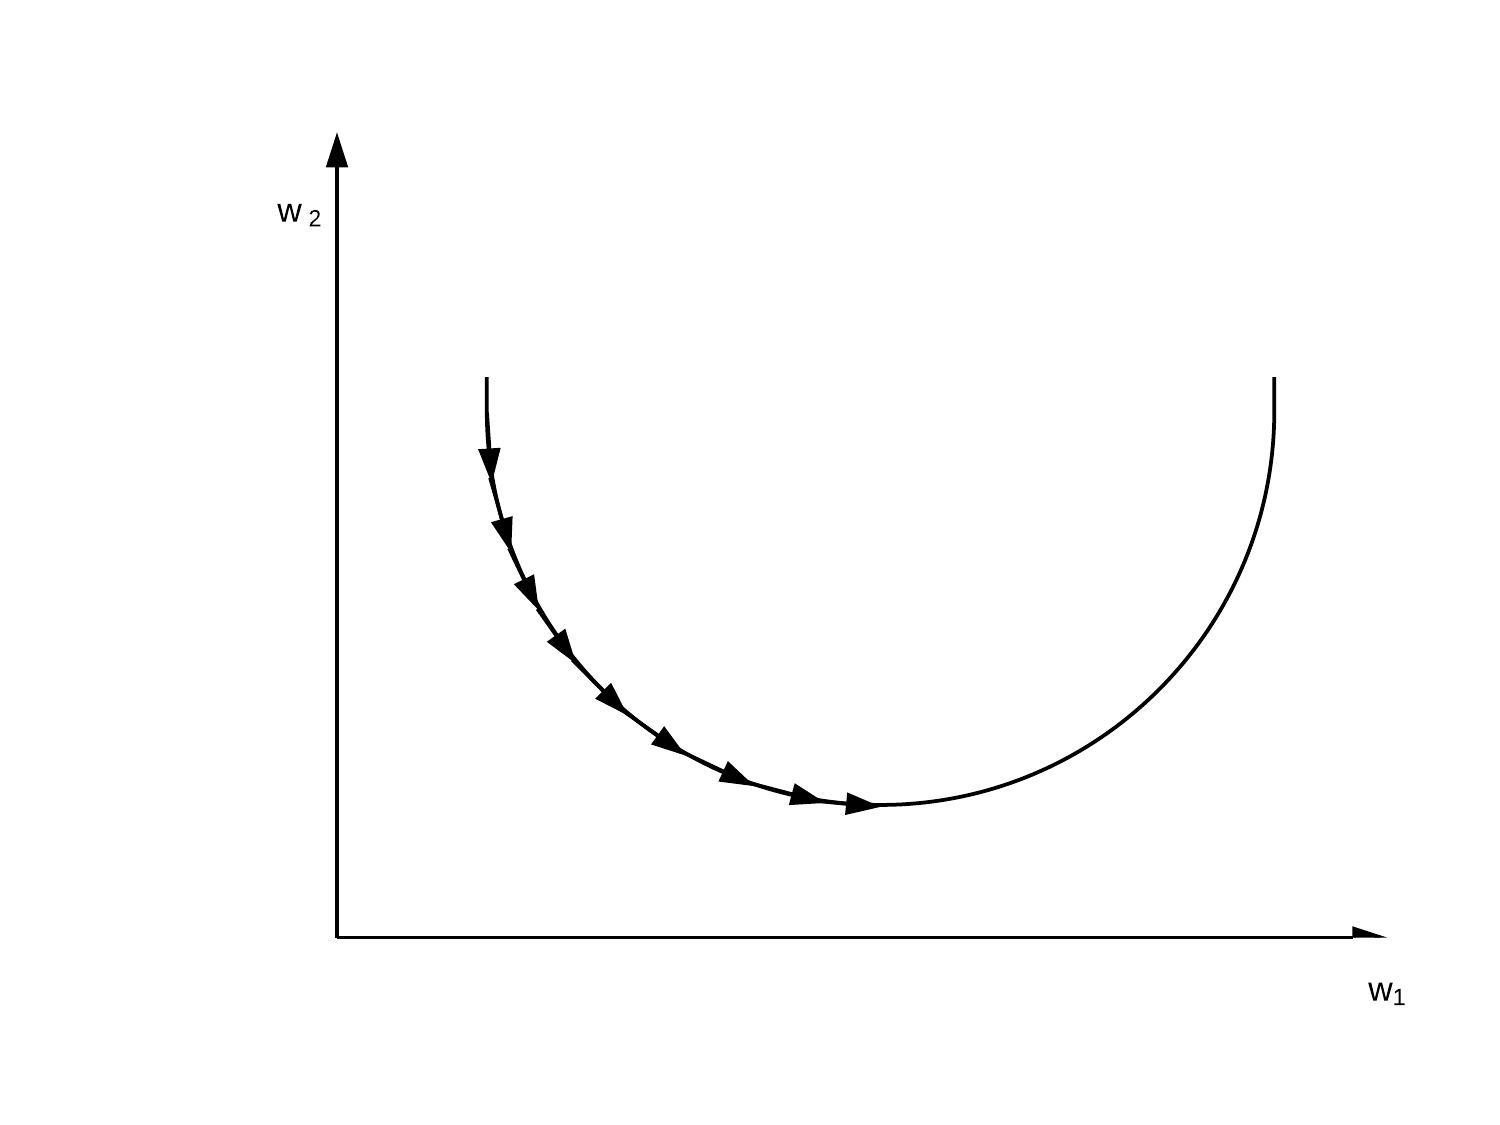
\includegraphics[width=\linewidth]{figuras/Sem_momentum.jpeg}
    \caption{Sem momentum}
  \end{subfigure}
  \begin{subfigure}[b]{0.4\linewidth}
    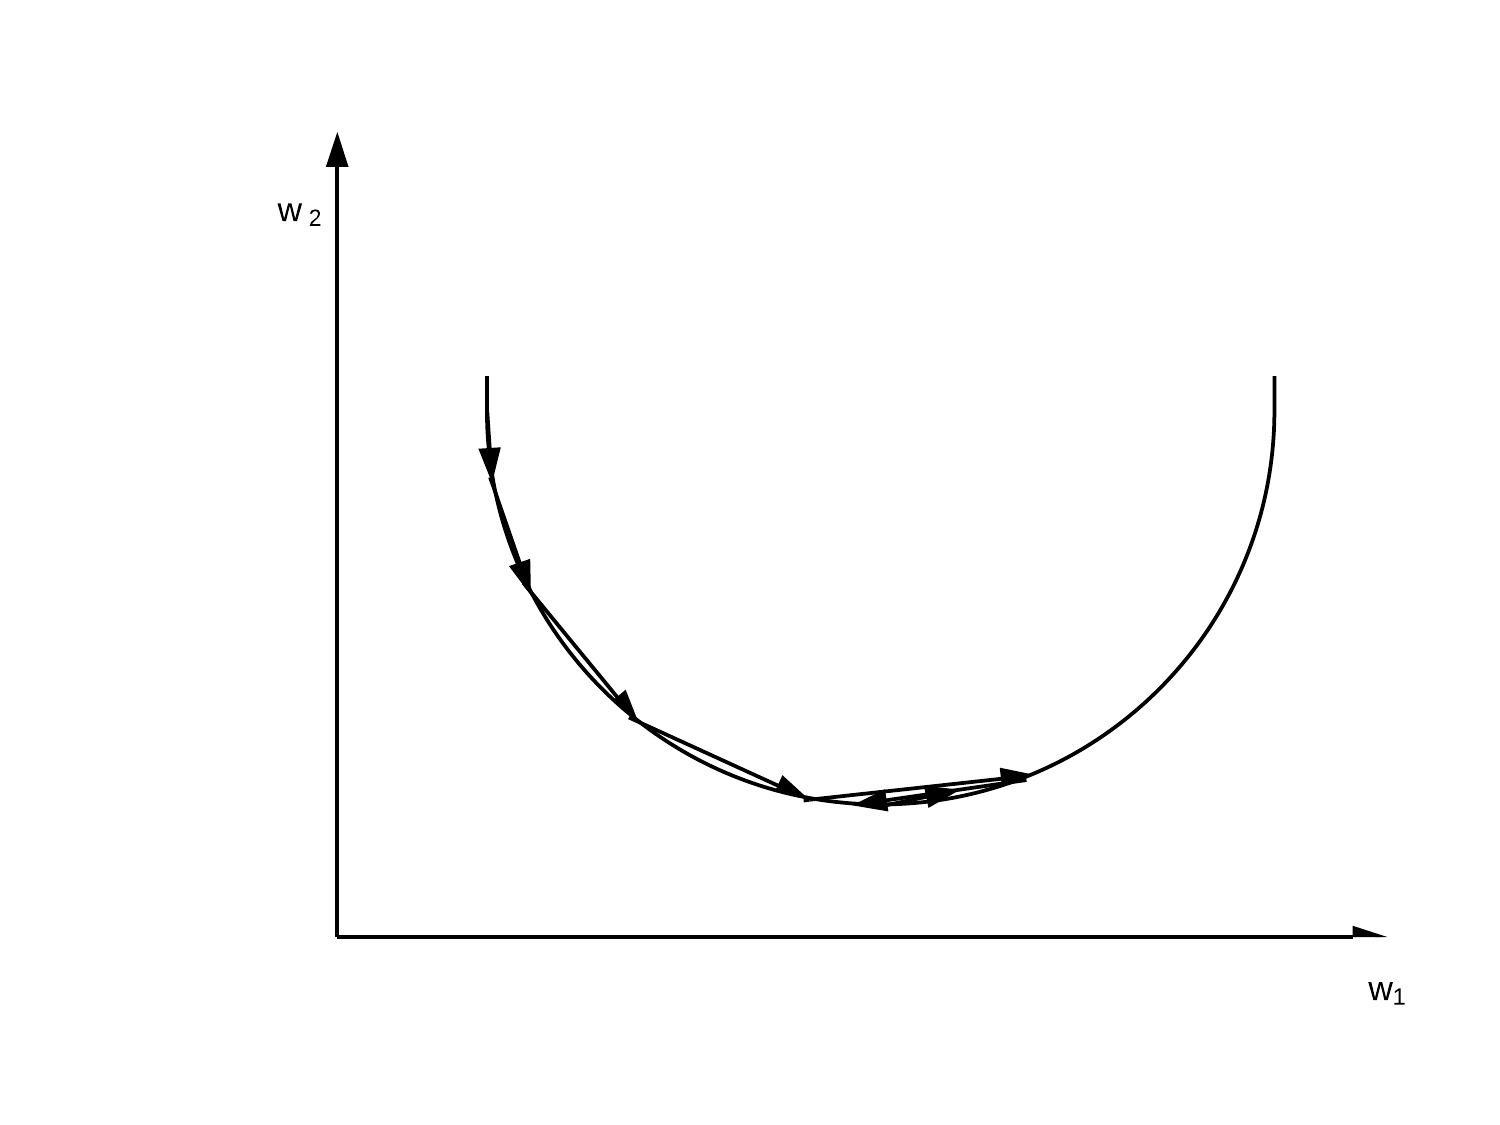
\includegraphics[width=\linewidth]{figuras/Com_momentum.jpeg}
    \caption{Com momemtum}
  \end{subfigure}
  \caption{Comparação de uso de momentum}
  \label{fig:coffee}
\end{figure}

Sabe-se que $\delta_j(n)y_i(n)$ é dado por $\frac{-\partial e(n)}{\partial w_{ij}(n)}$. Quando esta derivada em particular tem o mesmo sinal em várias iterações sucessivas, o ajuste de $\Delta w_{ij}(n)$ cresce, portanto a inclusão do momentum tende a acelerar o aprendizado.

Quando a derivada $\frac{\delta e(n)}{\delta w_{ij}(n)}$ tem o sinal oposto em iterações sucessivas, o ajuste diminui. Portanto a inclusão do momentum tende a estabilizar o efeito de oscilação durante o aprendizado.

\section{Validação Cruzada}

\begin{figure}[H]
  \centering
  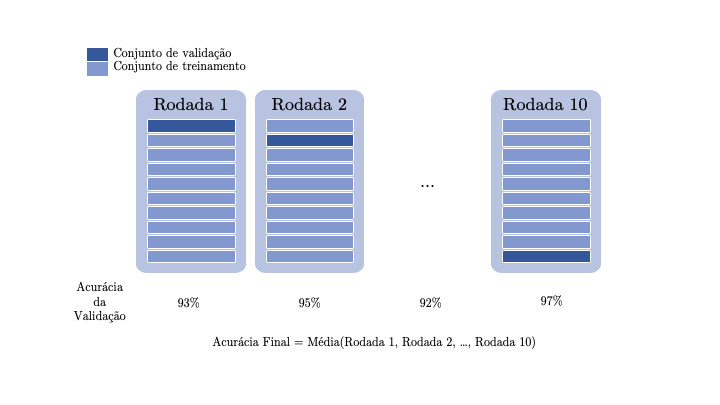
\includegraphics[width=450pt]{figuras/validacao_cruzada.png}
  \caption{Ilustração de multi-pastas no método de validação cruzada. Para uma rodada, o subconjunto dos dados destacados azul escuro é usado para validar o modelo treinado com o restante dos dados.}
  \label{fig:validacao_cruzada}
\end{figure}

Em essência o algoritmo de retropropagação codifica um mapeamento entrada-saída em uma rede neural perceptron de múltiplas camadas. Espera-se que a rede seja tão bem treinada com os dados passados, que consiga generalizar o futuro. Nessa perspectiva, o processo de aprendizado envolve encontrar o conjunto de parâmetros ou estrutura de acordo com um certo critério.

Uma ferramenta/técnica estatística conhecida como validação cruzada \cite{stone1974cross} permite testar o modelo com um conjunto de dados diferente do qual foi usado para parametrizar a rede neural.

Para isso, ordena-se o conjunto de dados de forma aleatória que é então dividido em amostra de treinamento e conjunto de teste. A amostra de treinamento é então particionada em dois conjuntos disjuntos:

\begin{itemize}
    \item um subconjunto de estimação usado para parametrizar o modelo
    \item um subconjunto de validação usado para testar/validar o modelo
\end{itemize}

Testar o modelo com o sub-conjunto de teste previne que o modelo seja incapaz de generalizar.
O problema então é como determinar o parâmetro $r$ que determine a divisão da amostra de treinamento entre o subconjunto de estimação e o subconjunto de validação. Em um estudo \cite{kearns1996bound} foi identificado que o valor $0.1$ funciona de maneira quase ótima para uma grande variedade de cenários. Ou seja, $90\%$ do conjunto de dados é destinado ao subconjunto de estimação e o restante $10\%$ é destinado ao subconjunto de validação.

\chapter{REDE NEURAL \& TRANSPORTE DE VALE}
No capítulo \ref{cap:redesneuraisempoucaspalavras} foram explicados os principais conceitos relacionados a redes neurais e como estes afetam o treinamento. Como explicado na introdução, as redes neurais podem ser treinadas para diversas tarefas específicas. O objetivo deste trabalho é encontrar modelar uma RNA que seja capaz de aprender a relação entre as configurações físicas de uma nanofita de grafeno, a energia imposta sobre ela e a transmissão de vale. Dessa forma, espera-se que a RNA seja capaz de determinar a transmissão de vale para configurações de nanofitas de grafeno não conhecidas pela RNA. 
Este objetivo pode ser modelado como um problema supervisionado de regressão numérica, mais especificamente uma aproximação de função \cite{cybenko1989approximation, hornik1989multilayer} cujas entradas são as configurações da nanofita de grafeno e energia e cuja saída seja a transmissão de vale. Considerando as entradas como um vetor \textbf{$x$} e a saída como \textbf{$d$}, tem-se:
\begin{equation*}
    d=f(x)
\end{equation*}
Um conjunto de dados de treinamento $T$ contendo os valores conhecidos de transmissão de dados e as configurações da nanofita de grafeno é dado, portanto tem-se:
\begin{equation}
\label{eqn:conjuntoTreinamento}
    T = {(x_i,d_i)}^N_{i=1} 
\end{equation}
Finalmente espera-se que a função $F(x)$ seja dada pela RNA e que descreva o mapeamento entrada-saída próximo o bastante de $f(x)$ no que diz respeito ao espaço euclidiano sobre todas as entradas, portanto tem-se:
\begin{equation*}
    ||F(x) - f(x)|| < \epsilon \text{ para todo } x
\end{equation*}
onde $\epsilon$ é um número positivo pequeno uma vez que $T$ é grande o bastante e que a rede é configurada com adequados hiperparâmetros.
A habilidade de uma rede neural de aproximar um mapeamento desconhecido entrada-saída pode ser analisado de duas formas:

\begin{itemize}
    \item Identificação de sistema: Usando o conjunto de treinamento \ref{eqn:conjuntoTreinamento} e dado que $y_i$ o vetor de saída para o vetor de entradas $x_i$, treina-se uma rede neural que minimiza o erro ($\epsilon$) dada a diferença dos quadrados entre $d_i$ e $y_i$ e ajusta os seus parâmetros livres (pesos e biases) de acordo com o $\epsilon$ encontrado na computação de todo o conjundo de treinamento $T$.
    \item Modelagem inversa: Quando deseja-se construir um \textit{modelo inverso} que produz o vetor \textbf{$x$} em resposta a um vetor $d$. O sistema inverso pode ser descrito por:
    \begin{equation*}
        x=f^{-1}(d)
    \end{equation*}
    Onde $f^{-1}(.)$ detona o inverso da função $f(.)$. Em muitas situações $f^{-1}(x)$ não é uma função facilmente calculável e por isso o uso de RNA se faz necessário, pois com ela espera-se encontrar uma aproximação de $f^{-1}(.)$. Neste caso, o vetor de entrada é $d_i$ e o vetor $x_i$ é tratado como resposta esperada. Da mesma maneira que em \textit{Identificação de sistema}, o $\epsilon$ é erro usado para ajustar os parâmetros livres da RNA a qual tenta minimizar a diferenças dos quadrados entre as saídas do sistema inverso desconhecido e a RNA. Tipicamente \textit{Modelagem Inversa} é uma tarefa de aprendizado mais difícil que \textit{Identificação de sistema} uma vez possivelmente não haja apenas uma única solução.
\end{itemize}

A seguir serão apresentadas algumas técnicas que facilitam a fase de treinamento tornando o processo de aprendizado mais rápido.

\section{Heurísticas para uma melhor performance do algoritmo de retropropagação}
Dizem que fazer o design é mais uma arte do que ciência. Isso acontece porque o resultado depende muito das experiências das pessoas, do conjunto de dados etc. Em parte isso é verdade, porém há algums métodos que ajudam uma rede neural a ter melhor performance. Abaixo serão explicados os métodos e fatores que influenciaram no experimento de treinar uma rede neural capaz de predizer o transporte de vale em nanofitas de grafeno deformada por gaussianas.

\subsection{Atualização em batch (lote) versus atualização estocástica}
O modo estocástico (sequencial) implica que os pesos sinápticos da rede neural são atualizados de acordo com cada exemplar do conjunto de treinamento. Ele é computacionalmente mais rápido que o modo em batch principalmente quando o conjunto de treinamento é grande e redundante, ou seja, que possui exemplares repetidos. Dados altamente redundantes acabam deixando o cálculo da matriz Jacobiana (necessária para atualização em lote) mais complexo.

\subsection{Conjunto de treinamento com máxima informação}
Como regra geral, todo exemplar de treinamento apresentado ao algoritmo de retropropagação deve ser escolhido com base na quantidade máxima de informação possível para o treinamento em questão (LeCun, \citeyear{lecun1993efficient}). Há duas maneiras de fazer isso:

\begin{itemize}
    \item Usar um exemplar que resulte no maior erro de treinamento.
    
    \item Usar um exemplar que seja radicalmente diferente de todos os outros previamente apresentados ao algoritmo.
\end{itemize}

Essas duas heurísticas são motivadas pelo desejo de se ter uma maior busca no espaço de pesos. Um método simples e comumente usado é ordenar de forma aleatória o conjunto de treinamento de forma a minimizar as chances de que exemplares similares sejam apresentados ao algoritmo. 

\subsection{Função de ativação}
No que diz respeito a velocidade de aprendizado, é preferível usar uma função de ativação do tipo sigmoid e que seja impar ao seu parâmeto, ou seja $\phi(-x)=-\phi(x)$. A função tangente hiperbólica, com as constantes $a=1.7159$ e $b=\frac{2}{3}$  satisfaz essa característica pois $\phi(1)=1$ e $\phi(-1)=-1$. Além disso, conforme mostrado abaixo, o ganho efetivo da função de ativação é próximo de $1$:

\begin{align*}
\phi(0) = & ab \\
= & 1.7159 \frac{2}{3} \\
= & 1.1424        
\end{align*}

\subsection{Atributos a serem preditos}
Os atributos a serem preditos, ou seja, a(s) saída(s) da rede neural precisam evitar os limites da função de ativação escolhida. Caso contrário, os pesos sinápticos tendem ao infinito diminuindo assim o processo de aprendizado ao colocar os neurônios das camadas ocultas em saturação. Como alternativa a usar a função de ativação com valores específicos citados acima para as constantes $a$ e $b$ da função de ativação, é sugerido pré-processar os dados de forma que evitem o limites, ou seja, a(s) resposta(s) desejada(s) da rede neural pode(m) estar compreendida(s) no intervalo [-0.9, 0.9]

\subsection{Normalização das entradas da rede neural}
Cada variável de entrada deve ser préprocessada de forma que sua média, ponderada sobre todo o conjunto de dados, seja próxima de zero ou que seja pequena se comparada a seu desvio padrão (LeCun,  \citeyear{lecun1993efficient}). Isso garante que os pesos na(s) camada(s) oculta(s) evitem a oscilação de direção na superfície de erro, acelerando assim o processo de aprendizado.

Além disso, as variáveis de entrada, se possível, não devem estar correlacionadas conforme mostrado na figura \ref{fig:correlacao}, onde é possível observar que exceto por a variável \textit{Transmissão}, a correlação está proxima de \textit{zero}. Isso é possível com o uso de análise de componentes principais.
Por fim, as variáveis de entrada devem ser normalizadas de forma que suas covarianças seja aproximadamente iguais, garantindo assim que os diferentes pesos sinápticos aprendam em velocidades similares.

\begin{figure}[H]
    \centering
  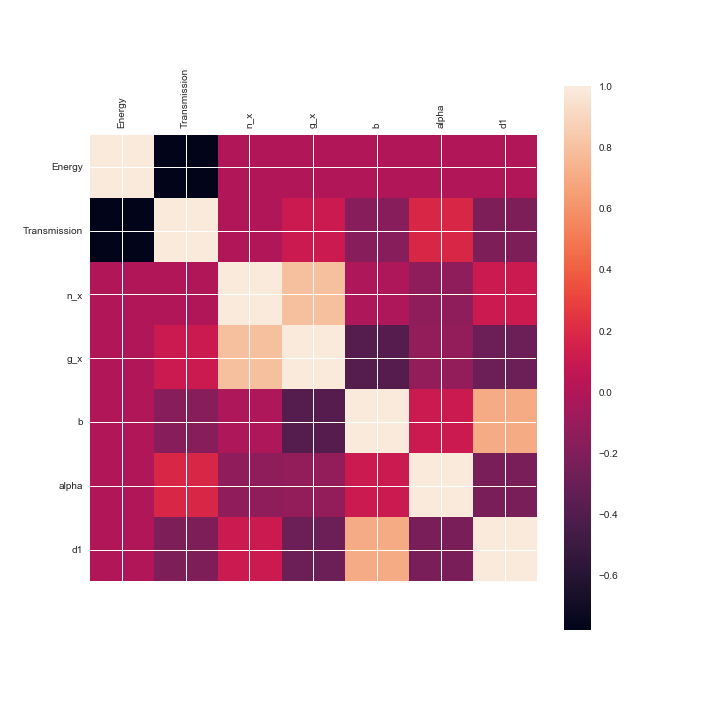
\includegraphics[width=300pt]{figuras/correlacao.png}
  \caption{Correlação das propriedades}
  \label{fig:correlacao}
\end{figure}

\subsection{Inicialização dos pesos sinápticos}

Após identificar os diversos parâmetros que descrevem as configurações físicas e influenciam nas propriedades eletrônicas em nanofita de grafeno, este trabalho faz o uso de rede neural artificial para descrever quantitativelmente os efeitos destes parâmetros na transmissão por vale. Detalhes destas atividades estão explicados nas seguintes sessões.

\section{Conjunto de dados e pré-processamento}
Os dados foram obtidos a partir de cálculos de  transporte eletrônico em nanofitas de grafeno com um número definido de deformações gaussianas. Eles foram estruturados em arquivos com extensões .txt e .dat. Estes arquivos foram então processados para gerar um único conjunto de dados que foi usado para treinar a rede neural artificial.
Cada arquivo .txt contém diversos parâmetros que descrevem as diferentes configuração físicas de nanofita de grafeno. Por exemplo, o arquivo com os seguintes pares de chave-valor foram analisados e a chave $n_y$ (número de átomos na direção vertical) com valor 70 resultou numa coluna cujos valores são iguais a 70. O mesmo foi feito para as chaves $n_x$ (número de átomos na direção vertical) com valor 2001 e $g_x$ (número de deformações gaussianas na direção horizontal) com valor 50.

\begin{table}[H]
\begin{minipage}{0.5\linewidth}
\caption{Conjunto chave-valor de configuração pré-processamento.}
\label{tab:chave_valores_preprocessamento}
\centering
\begin{tabular}{c|c}
\toprule
\textbf{Chave} & \textbf{Valor} \\
\midrule
\bm{$n_y$} & $70$    \\
\bm{$n_x$} & $2001$  \\
\bm{$g_x$} & $50$    \\
\textbf{b}   & $6ab$   \\
\bm{$d_1$}  & $20\sqrt{3}ac$   \\
\textbf{alpha}  & $22.2$\% \\
\bottomrule % <-- Bottomrule here
\end{tabular}
\end{minipage}
\begin{minipage}{0.5\linewidth}
\caption{Conjunto chave-valor de configuração pós processamento.}
\label{tab:chave_valores_posprocessamento}
\centering
\begin{tabular}{c|c}
\toprule
\textbf{Chave} & \textbf{Valor} \\
\midrule
\bm{$n_y$} & 70    \\
\bm{$n_x$} & 2001  \\
\bm{$g_x$} & 50    \\
\textbf{b}   & $0,0852$   \\
\bm{$d_1$}  & $4,919$   \\
\textbf{alpha}  & $0.222$\% \\
\bottomrule % <-- Bottomrule here
\end{tabular}
\end{minipage}
\end{table}

O mesmo foi feito com a chave b (desvio padrão das bases das deformações gaussianas) com o valor $6*ac$, mas um cálculo adicional foi feito devido a dependência no valor de $ac$ que é uma constante de distância entre os átomos de carbono valor $0.142nm$. Neste caso, a chave $b$ resultou numa coluna cujos valores são iguais a $6*0.142nm = 0,0852$. A chave $d1$ (distância entre cada deformação gaussiana) com o valor $20*\sqrt{3}*ac$ resultou em uma coluna cujos valores são iguais a $20*\sqrt{3}*0.142nm=4,919$. A chave $alpha$ (parâmetro de pressão da gaussiana) com o valor $22.2\%$ resultou numa coluna com valores iguais a $0.222$.

Um pouco de informação sobre o conjunto de dados:

\begin{table}[H]
    \begin{center}
    \caption{Descrição das propriedades envolvidas no experimento}
    \label{tab:Descrição das propriedades do grafeno}
    \resizebox{16cm}{!}{
    \begin{tabular}{ l | l }
    \toprule
	\textbf{Propriedade} & \textbf{Descrição} \\ 
	\midrule
    \bm{$n_x$} & número de átomos no eixo X, ou seja, é o comprimento da nanofita \\
    \bm{$n_y$} & número de átomos no eixo Y, ou seja, é a largura da nanofita  \\
    \bm{$g_x$} & número de deformações gaussianas ao longo do eixo X na nanofita de grafno \\
    \bm{$d_1$} & distância os centros de deformações gaussianas vizinhas na nanofita de grafeno \\
    \textbf{b} & largura das deformações gaussiana \\
    \textbf{alpha} & relação entre a altura e a largura da deformações gaussianas, ou seja, $\alpha = (A/b)^2$. Está relacionado com o \textit{strain} produzido por uma deformação gaussiana \\
    \textbf{Energy} & energia dos elétrons incidentes \\
    \textbf{Conductance} & condutância elétrica $G(2e^2/h)$ \\
    \textbf{Transmission} & probabilidade de transmissão por vale \\
    \bottomrule % <-- Bottomrule here
    \end{tabular}
    }
    \end{center}
\end{table}

Os dados foram estatisticamente descritos abaixo:

\begin{table}[h!]
  \begin{center}
    \caption{Análise estatística dos dados.}
    \label{tab:analise_estatistica_dados}
    \resizebox{16cm}{!}{
    \begin{tabular}{l | S | S | S | S | S | S | S | S | S}
      \toprule
      \textbf{Function} & \textbf{Energy} & \textbf{Conductance} & \textbf{Transmission} & \bm{$n_x$} & \bm{$n_y$} & \bm{$g_x$} & \textbf{b} & \textbf{alpha} & \bm{$d_1$} \\
      \midrule
	count & 59000.00 & 59000.00 & 59000.00 & 59000.00 & 59000.00 & 59000.00 & 59000.00 & 59000.00 & 59000.00 \\
	mean & 0.25 & 8.28 & 0.67 & 1257.76 & 73.81 & 12.13 & 3.06 & 14.34 & 11.64 \\ 
	std & 0.14 & 7.39 & 0.18 & 769.00 & 20.94 & 8.61 & 0.59 & 12.88 & 2.83 \\ 
	min & 0.001 & 0.60 & 0.49 & 40.00 & 20.00 & 0.00 & 0.85 & 0.00 & 4.90 \\ 
	0.25 & 0.12 & 2.11 & 0.53 & 801.00 & 70.00 & 7.00 & 3.12 & 1.00 & 11.07 \\ 
	0.5& 0.25 & 6.33 & 0.57 & 1145.00 & 70.00 & 11.00 & 3.12 & 13.00 & 11.07 \\ 
	0.75 & 0.37 & 12.78 & 0.73 & 1801.00 & 70.00 & 17.00 & 3.12 & 25.00 & 11.07 \\ 
	max & 0.50 & 48.92 & 1.00 & 3601.00 & 150.00 & 60.00 & 4.54 & 40.00 & 22.13 \\ 
      \bottomrule % <-- Bottomrule here
    \end{tabular}
    }
  \end{center}
\end{table}



% \section{Centralizar as variáveis de entrada}
% \section{Normalização dos dados}
% \section{Descorrelacionar variáveis de entrada}
% \section{Definição da função de ativação}
% \section{Escalar os dados de saída para o intervalo da função de ativação}
% \section{Inicialização dos pesos}
% \section{Uso de gradiente conjugado para regressão}


% A rede neural calcula uma função $M( Zˆp , W )$, onde $Z^p$ é o p-ésimo padrão de entrada, e $W$ representa o conjunto de parâmetros ajustáveis no sistema. A função de custo  $E^p=\frac{1}{2}(D^p,M(Z^p,W))^2$ mede a discrepância entre a saída ``correta'' ou esperada $D^p$ para o padrão de entrada $Z^p$ e a saída produzida pelo sistema. A função de custo médio $E_{treino}(W)$ é a média dos erros $E^{p}$ sobre um conjunto de pares $\{(D^1,Z^1),...(D^P,Z^P)\}$. A performance é estimada em um conjunto de dados disjunto do conjunto de dados de treinamento, chamado conjunto de teste. A função de custo mais comumente usada é erro quadrático médio.

As estratégias usadas nesta sessão buscam não somente minimizar a função de custo, mas melhorar a capacidade da rede neural de generalizar, isto é, de predizer valores para padrões não previamente apresentados à rede neural.

$$E_{treino}=\frac{1}{P} \sum_{p=1}^P E^p$$ 

Uma vez que rede neural artificial foi usada neste experimento, os dados precisam ser preparados para tal.
A maioria dos valores são maiores que 1, portanto os valores foram escalados no intervalo $[-0.9, 0.9]$ de forma a acelerar o processo de treinamento da RNA.

Os dados escalados estão estatisticamente descritos abaixo:

\begin{figure}
    \centering
    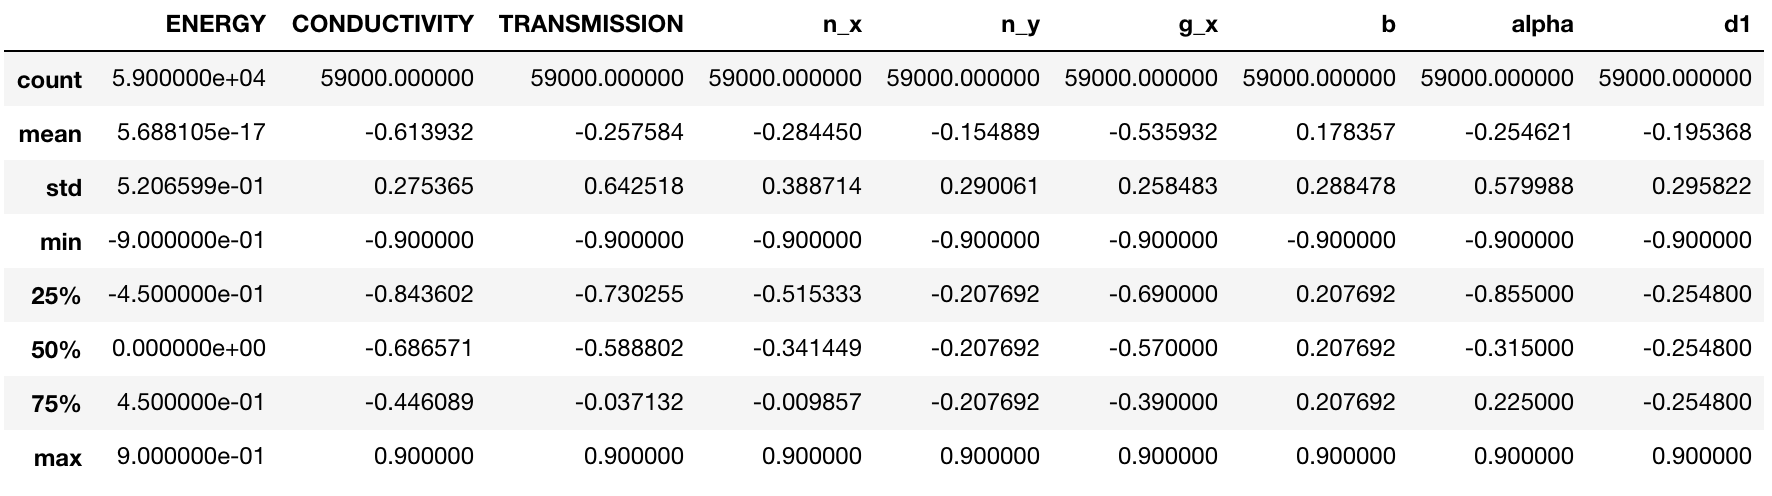
\includegraphics[width=350px]{figuras/scaled_data_summary.png}
    \caption{Descrição estatística dos dados escalados}
    \label{fig:Scaled data summary}
\end{figure}

\begin{figure}
    \centering
    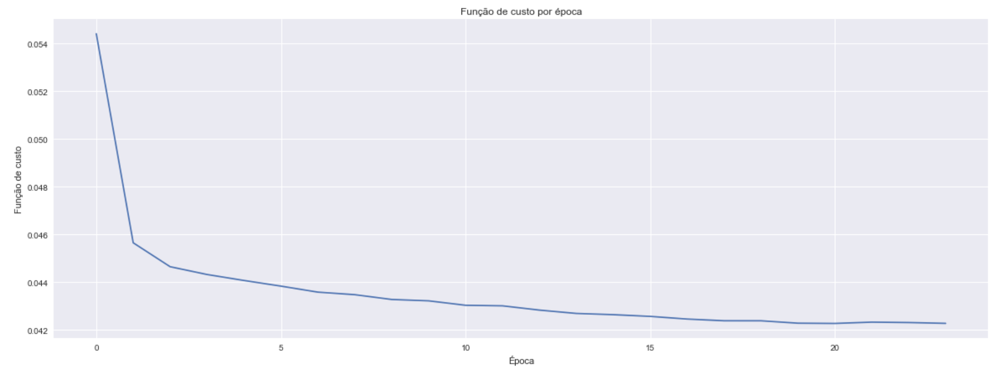
\includegraphics[width=350px]{figuras/erro_por_epoca.png}
    \caption{Função de erro por época de treinamento}
    \label{fig:Loss function per epoch}
\end{figure}

Cada arquivo .dat contém três colunas: energia($E/t$), condutância elétrica ($G(2e^2)/h)$) e transmissão por vale.

\sisetup{
  round-mode          = places, % Rounds numbers
  round-precision     = 3, % to 2 places
}

\begin{table}[h!]
    \begin{center}
    \caption{Análise de $R^2$ e RMSE por conjunto de parâmetros da MLP; $\eta$: Taxa de aprendizado; N: Neurônios na camada oculta; C: Condutância; T: Transmissão; val: validação; tre: treino; tes: teste.}
    \label{tab:analise_performance_mlp.}
    \resizebox{16cm}{!}{
    \begin{tabular}{ r | S |  S | S | S | S | S | S | S | S | S }
    \toprule
	\bm{$\eta$} & \textbf{N} & \textbf{R2 [tre]} & \textbf{RMSE C. [tre]} & \textbf{RMSE T. [tre]} & \textbf{R2 [val]} & \textbf{RMSE C. [val]} & \textbf{RMSE T. [val]} & \textbf{R2 [tes]} & \textbf{RMSE C. [tes]} & \textbf{RMSE T. [tes]} \\ 
	\midrule
0.01 & 50                         & 0.851880        & 0.075278                     & 0.274369                      & 0.847142           & 0.078587                        & 0.280333                         & 0.847591       & 0.077651                    & 0.278660                     \\
0.01 & 10                         & 0.853864        & 0.074270                     & 0.272525                      & 0.844657           & 0.079864                        & 0.282602                         & 0.843599       & 0.079685                    & 0.282286                     \\
0.01 & {(10, 10, 10)}               & 0.859360        & 0.071477                     & 0.267351                      & 0.859130           & 0.072423                        & 0.269116                         & 0.859277       & 0.071698                    & 0.267764                     \\
0.10 & 10                         & 0.859430        & 0.071441                     & 0.267285                      & 0.855857           & 0.074106                        & 0.272224                         & 0.860639       & 0.071004                    & 0.266465                     \\
0.10 & 50                         & 0.860539        & 0.070878                     & 0.266229                      & 0.853301           & 0.075420                        & 0.274627                         & 0.852997       & 0.074897                    & 0.273673                     \\
0.01 & {(10, 10)}                   & 0.864723        & 0.068751                     & 0.262205                      & 0.859285           & 0.072344                        & 0.268968                         & 0.858999       & 0.071839                    & 0.268028                     \\
0.01 & {(50, 50)}                   & 0.867618        & 0.067280                     & 0.259383                      & 0.860371           & 0.071785                        & 0.267928                         & 0.860841       & 0.070901                    & 0.266272                     \\
0.01 & {(50, 50, 50)}               & 0.875364        & 0.063343                     & 0.251681                      & 0.863935           & 0.069953                        & 0.264486                         & 0.865086       & 0.068738                    & 0.262179                     \\
0.10 & {(50, 50)}                   & 0.875471        & 0.063289                     & 0.251572                      & 0.864361           & 0.069734                        & 0.264072                         & 0.865918       & 0.068314                    & 0.261370                     \\
0.10 & {(10, 10, 10)}               & 0.877688        & 0.062162                     & 0.249323                      & 0.864821           & 0.069497                        & 0.263624                         & 0.865710       & 0.068420                    & 0.261572                     \\
0.10 & {(10, 10)}                   & 0.880147        & 0.060912                     & 0.246804                      & 0.860660           & 0.071637                        & 0.267650                         & 0.871035       & 0.065707                    & 0.256334                     \\
0.10 & {(50, 50, 50)}               & 0.894069        & 0.053837                     & 0.232028                      & 0.875658           & 0.063926                        & 0.252836                         & 0.872585       & 0.064917                    & 0.254789      \\           
    \bottomrule % <-- Bottomrule here
    \end{tabular}
    }
    \end{center}
\end{table}

\begin{table}[H]
\centering
\caption{Parâmetros que definem a estrutura da MLP já treinada.}
\label{parametros_rede_treinada}
\begin{tabular}{ r | l }
\toprule
\textbf{Especificação} & \textbf{Valor} \\
\midrule
Rede Neural & Perceptron de multiplas camadas \\
Função de ativação & tangente hiperbólica \\
Taxa de aprendizado & 0.10 \\
Momentum & 0.90 \\
Número de camadas ocultas & 1.00 \\
Número de nós na camada oculta & {(50,50,50)} \\
Número de nós na camada de entrada  & 6.00 \\
Número de nós na camada de saída & 1.00 \\
Algorítimo  & gradiente estocástico descendente \\
\bottomrule
\end{tabular}
\end{table}

\section{Modelagem de rede neural artificial e parametrização}
Na primeira etapa os dados pré-processados foram ordenados de foram aleatória e divididos em conjunto de treinamento, validação e teste. A porcentagem de observações por conjunto é de 60\%, 20\% e 20\%, para os conjuntos de treinamento, validação e teste, respectivamente. O conjunto de treinamento foi usado para treinar a Rede Neural Artificial (RNA). Os  dados de validação foi usado em conjunto com o dados de treinamento para determinar quando interromper o processo de aprendizado, de modo que o modelo resultante exibisse boas métricas de generalização. Os dados de teste permitem a avaliação das capacidades de predição do modelo de RNA. A RNA foi avaliada usando como
critérios de desempenho o erro quadrado médio (MSE) e o coeficiente de determinação ($R^2$) sobre os conjuntos de dados de treinamento e teste.

\todo{Rever esta parte}

A seguinte etapa se refere a configuração e a otimização da arquitetura de RNA. O modelo de RNA foi projetado com três camadas: uma camada de entrada, uma
camada oculta e uma camada de saída. De um modo geral, uma camada oculta é suficiente para a maioria dos problemas práticos de regressão, portanto, apenas uma camada oculta foi usada neste estudo. O desempenho da RNA foi testado com mais de uma camada oculta.
A quantidade de nós na camada de entrada e saída da RNA foram definidos de acordo com o número de fatores/atributos de entrada e o número de variáveis a serem previstas. A camada de entrada tem nove nós que representam as seis chaves supracitadas além das propriedades energia, condutância elétrica e transmissão por vale. Uma busca exaustiva foi realizada para determinar o número ideal de neurônios na camada oculta, a taxa de aprendizado, o algorítmo de aprendizado, a função de ativação / saída, momentum e alpha de acordo com os critérios de desempenho supracitados.

% \section{Análise de desempenho e erro da rede neural}

% \section{Análise gráfica dos erros nos subconjuntos de treino, validação e teste}

\section{Arquitetura da rede neural treinada}

A estrutura final do modelo da RNA possui 50 neurônios em cada camada oculta. A função de ativação da camada oculta e na camada de saída do modelo é a função tangente hiperbólica. O processo de treinamento foi conduzido utilizando o algoritmo padrão de retropropagação (gradiente estocástico descendente) como procedimento de otimização, com pesos atualizados a cada vez que o conjunto completo de dados de treinamento foi considerado.
O modelo de RNA obteve um bom desempenho nos dados de treinamento / validação / teste, com um valor de $R^2$ de ~ $0.909$ para cada. A RNA desempenhou satisfatoriamente para todo o conjunto de dados. Deve-se perceber que esse modelo de RNA não considera outros fatores que possam afetar os valores de transmissão por vale. O conjunto de dados que suporta o modelo de RNA é limitado às condições investigadas neste experimento. Devido à sua natureza orientada por dados, o modelo de RNA pode ser melhorado progressivamente, treinando-o com mais dados observados.

% PRE-PROCESSAMENTO
% 1-Discretização
% 2-Normalização/Scale the data
% MODELAGEM DE REDE NEURAL
% 

% \section{REFERÊNCIAS BIBLIOGRÁFICAS}


% ----------------------------------------------------------
% Finaliza a parte no bookmark do PDF
% para que se inicie o bookmark na raiz
% e adiciona espaço de parte no Sumário
% ----------------------------------------------------------
\phantompart

\postextual
% ----------------------------------------------------------

% ----------------------------------------------------------
% Referências bibliográficas
% ----------------------------------------------------------


% \bibliographystyle{abnt-alf}
\bibliography{references.bib}

\end{document}